\documentclass[aps,prd,reprint,superscriptaddress]{revtex4-2}

\usepackage[utf8]{inputenc}
\usepackage[T1]{fontenc}
\usepackage{graphicx}
\usepackage{siunitx}
\usepackage{subcaption}
\usepackage[colorlinks=true,
            linkcolor=blue,
            citecolor=blue,
            urlcolor=blue]{hyperref}
\usepackage{url}
\usepackage{booktabs}
\usepackage{amsmath,amsfonts}
\usepackage{nicefrac}
\usepackage{microtype}
\usepackage{xcolor}
%\usepackage{stfloats}  % allows bottom placement for two-column floats
\usepackage{listings}
\usepackage{listings-ext}

\lstset{
    language=Python,                  % Or remove this if you do not want highlighting
    frame=single,
    breaklines=true,
    %breakanywhere=true,               % Wrap inside words if needed
    basicstyle=\ttfamily\scriptsize,  % Small font often fits logs better
    columns=fullflexible,
    backgroundcolor=\color{gray!10},
    keepspaces=true                   % Preserve spaces
}


\begin{document}

\makeatletter
\renewcommand\@makecaption[2]{%
  \small\rmfamily
  \begin{list}{}{%
      \setlength{\leftmargin}{0pt}%
      \setlength{\rightmargin}{0pt}%
    }%
    \item[]\textbf{#1:} #2%
  \end{list}%
}
\makeatother

\title{Automating High Energy Physics Data Analysis with LLM-Powered Agents}

% \author{Haichen Wang}
% \email{haichenwang@berkeley.edu}
% \affiliation{Department of Physics, University of California, Berkeley, Berkeley, CA 94720, USA}
% \affiliation{Physics Division, Lawrence Berkeley National Laboratory, Berkeley, CA 94720, USA}

% \author{Dongwon Kim}
% \email{dwkim@berkeley.edu}
% \affiliation{Department of Physics, University of California, Berkeley, Berkeley, CA 94720, USA}
% \affiliation{Physics Division, Lawrence Berkeley National Laboratory, Berkeley, CA 94720, USA}

% \author{Joshua Ho}
% \email{ho22joshua@berkeley.edu}
% \affiliation{Department of Physics, University of California, Berkeley, Berkeley, CA 94720, USA}
% \affiliation{Physics Division, Lawrence Berkeley National Laboratory, Berkeley, CA 94720, USA}

% \author{Luc Tomas Le Pottier}
% \email{luclepot@berkeley.edu}
% \affiliation{Department of Physics, University of California, Berkeley, Berkeley, CA 94720, USA}
% \affiliation{Physics Division, Lawrence Berkeley National Laboratory, Berkeley, CA 94720, USA}

% \author{Chengxi Yang}
% \email{cxyang@berkeley.edu}
% \affiliation{Department of Physics, University of California, Berkeley, Berkeley, CA 94720, USA}
% \affiliation{Physics Division, Lawrence Berkeley National Laboratory, Berkeley, CA 94720, USA}

% \author{Eli Gendreau-Distler}
% \email{egendreaudistler@berkeley.edu}
% \affiliation{Department of Physics, University of California, Berkeley, Berkeley, CA 94720, USA}
% \affiliation{Physics Division, Lawrence Berkeley National Laboratory, Berkeley, CA 94720, USA}
\author{Eli Gendreau-Distler}
\email{egendreaudistler@berkeley.edu}
\affiliation{Department of Physics, University of California, Berkeley, Berkeley, CA 94720, USA}
\affiliation{Physics Division, Lawrence Berkeley National Laboratory, Berkeley, CA 94720, USA}

\author{Joshua Ho}
\email{ho22joshua@berkeley.edu}
\affiliation{Department of Physics, University of California, Berkeley, Berkeley, CA 94720, USA}
\affiliation{Physics Division, Lawrence Berkeley National Laboratory, Berkeley, CA 94720, USA}

\author{Dongwon Kim}
\email{dwkim@berkeley.edu}
\affiliation{Department of Physics, University of California, Berkeley, Berkeley, CA 94720, USA}
\affiliation{Physics Division, Lawrence Berkeley National Laboratory, Berkeley, CA 94720, USA}

\author{Luc Tomas Le Pottier}
\email{luclepot@berkeley.edu}
\affiliation{Department of Physics, University of California, Berkeley, Berkeley, CA 94720, USA}
\affiliation{Physics Division, Lawrence Berkeley National Laboratory, Berkeley, CA 94720, USA}

\author{Haichen Wang}
\email{haichenwang@berkeley.edu}
\affiliation{Department of Physics, University of California, Berkeley, Berkeley, CA 94720, USA}
\affiliation{Physics Division, Lawrence Berkeley National Laboratory, Berkeley, CA 94720, USA}

\author{Chengxi Yang}
\email{cxyang@berkeley.edu}
\affiliation{Department of Physics, University of California, Berkeley, Berkeley, CA 94720, USA}
\affiliation{Physics Division, Lawrence Berkeley National Laboratory, Berkeley, CA 94720, USA}

\begin{abstract}
We present a proof-of-principle study demonstrating the use of large language model (LLM) agents to automate a representative high energy physics (HEP) analysis. Using the Higgs boson diphoton cross-section measurement as a case study with ATLAS Open Data, we design a hybrid system that combines an LLM-based supervisor–coder agent with the \texttt{Snakemake} workflow manager. In this architecture, the workflow manager enforces reproducibility and determinism, while the agent autonomously generates, executes, and iteratively corrects analysis code in response to user instructions. We define quantitative evaluation metrics -- success rate, error distribution, costs per specific task, and average number of API call for the task -- to assess agent performance across multi-stage workflows. To characterize variability across architectures, we benchmark a representative selection of state-of-the-art LLMs, spanning the \textit{Gemini} and \textit{GPT-5} series, the \textit{Claude} family, and leading open-weight models.  While the workflow manager ensures deterministic execution of all analysis steps, the final outputs still show stochastic variation. Although we set the temperature to zero, other sampling parameters (e.g., top-p, top-k) remained at their defaults, and some reasoning-oriented models internally adjust these settings. Consequently, the models do not produce fully deterministic results. This study establishes the first LLM-agent-driven automated data-analysis framework in HEP, enabling systematic benchmarking of model capabilities, stability, and limitations in real-world scientific computing environments. The baseline code used in this work is available at \href{https://huggingface.co/HWresearch/LLM4HEP}{https://huggingface.co/HWresearch/LLM4HEP}. This work was accepted as a poster at the Machine Learning and the Physical Sciences (ML4PS) workshop of the 39th Conference on Neural Information Processing Systems (NeurIPS 2025). The initial submission was made on August 30, 2025.
\end{abstract}
\maketitle

\section{Introduction}
Large language models (LLMs) and agent-based systems are increasingly being explored in scientific computing, with applications appearing in areas such as genomics and software engineering~\citep{xiao2024cellagentllmdrivenmultiagentframework,wang2025empiricalresearchutilizingllmbased}. 
Despite the inherently structured nature of collider-related data analyses and the potential advantages of automated, reproducible workflows, the usage of LLMs in high energy physics (HEP) is still at an early stage. 
Existing efforts in HEP have focused mainly on event-level inference or on domain-adapted language models~\citep{richmond2025feyntunelargelanguagemodels,simons2024astrohepbertbidirectionallanguagemodel,wu2024scalingparticlecollisiondata}, leaving open questions about how LLMs might participate directly in end-to-end analysis procedures.

Related work in agentic methodologies, including the \textit{Agents of Discovery} study~\citep{Diefenbacher:2025zzn}, demonstrates growing interest in structuring collider physics tasks through modular agent behavior. While such efforts examine agent-based reasoning in HEP contexts, they address different objectives and operational settings. Our study is situated within a workflow-management environment and considers how agentic components may be incorporated into a directed, reproducible analysis pipeline.

We introduce a framework in which LLM-based agents are integrated into a \texttt{Snakemake}-managed workflow~\citep{molder2021snakemake}. Agent interventions are bounded to well-defined tasks such as code generation, event selection, and validation while the underlying directed acyclic graph (DAG) maintains determinism and provenance. This design enables a controlled evaluation of the practicality and reliability of agent-driven steps within a full collider-analysis setting.

%While large language models (LLMs) and agentic systems have been explored for automating components of scientific discovery in fields such as biology (e.g., CellAgent for single-cell RNA-seq analysis~\citep{xiao2024cellagentllmdrivenmultiagentframework}) and software engineering (e.g., LangGraph-based bug fixing agents~\citep{wang2025empiricalresearchutilizingllmbased}), their application to high energy physics (HEP) remains largely unexplored. In HEP, analysis pipelines are highly structured, resource-intensive, and with strict requirements of reproducibility and statistical rigor. Existing work in HEP has primarily focused on machine learning models for event classification or simulation acceleration, and more recently on domain-adapted LLMs (e.g., FeynTune~\citep{richmond2025feyntunelargelanguagemodels}, Astro-HEP-BERT~\citep{simons2024astrohepbertbidirectionallanguagemodel}, BBT-Neutron~\citep{wu2024scalingparticlecollisiondata}) and conceptual roadmaps for large physics models. However, to the best of our knowledge, no published study has demonstrated an agentic system that autonomously generates, executes, validates, and iterates on HEP data analysis workflows.

%In parallel to our work, a related agent-based approach for HEP anomaly detection has been explored in the \textit{Agents of Discovery}~\citep{Diefenbacher:2025zzn} paper. While this reflects growing interest in applying agentic methodologies to HEP, the scope, workflow structure, and design choices differ markedly from those pursued here. In particular, the present work focuses on embedding a task-directed agent within a reproducible \texttt{Snakemake}-managed workflow and constraining agent behavior through a domain-specific directed acyclic graph (DAG). The methodological objectives and operational setting are therefore distinct and were developed independently.

%In this work, we present the first attempt to operationalize LLM-based agents within a reproducible HEP analysis pipeline. Our approach integrates a task-focused agent with the \texttt{Snakemake} workflow manager \citep{molder2021snakemake}, leveraging \texttt{Snakemake}’s HPC-native execution and file-based provenance to enforce determinism, while delegating bounded subtasks (e.g., event selection, code generation, validation, and self-correction) to an LLM agent. This design departs from prior agent frameworks such as LangChain~\citep{langchain2022} or LangGraph~\citep{langgraph2025} that emphasize flexible multi-step reasoning by embedding the agent within a domain-constrained DAG, ensuring both scientific reliability and AI relevance.

\section{Background and Motivation}
Research connecting LLMs with HEP is rapidly developing, though the existing literature remains concentrated on a small number of application areas -- for instance, enhancements to event-level prediction tasks, improvements to simulation, or tools for navigating domain knowledge. A substantial body of work applies transformer-based architectures to established HEP tasks such as classification, regression, and generative modeling~\citep{Qu:2022mxj,Qiu:2022xvr,Huang:2024voo,Mikuni:2024qsr}. These studies demonstrate the effectiveness of modern model architectures within conventional workflows but are not designed to automate or restructure the broader analysis process.
%Research connecting LLMs with HEP is rapidly developing, though the existing literature remains concentrated on only a few applications. A substantial body of work applies transformer-based architectures to established HEP tasks such as classification, regression, and generative modeling~\citep{Qu:2022mxj,Qiu:2022xvr,Huang:2024voo,Mikuni:2024qsr}. These studies demonstrate the effectiveness of modern model architectures within conventional workflows but are not designed to automate or restructure the broader analysis process.

LLMs have also been used to improve access to experiment-specific documentation and technical resources. Systems such as \texttt{Chatlas}~\citep{DalSanto:2935252}, \texttt{LLMTuner}~\citep{schnabel2025largelanguagemodelsnew}, and \texttt{Xiwu}~\citep{xiwu} demonstrate the usefulness of natural-language interfaces for accessing experiment-specific documentation and technical information. Their focus, however, is on retrieval and interpretation rather than direct interaction with analysis pipelines or workflow tools.

A further line of research examines the use of LLMs for code generation and the operation of scientific software. Examples include ChatGPT-assisted analysis scripting at the Electron–Ion Collider~\citep{eic} and the use of LLMs to configure and run FLUKA simulations~\citep{ndum2024autoflukalargelanguagemodel,fluka}. These demonstrations highlight that LLMs can interface with complex software environments, motivating exploration of more integrated, workflow-level applications.

Developments outside HEP provide additional context for an agent-based approach. Structured prompting has enabled LLMs to execute multi-step scientific procedures by decomposing tasks into modular operations~\citep{Pan2025LLMHF,reasoner,benchmark}. In parallel, lightweight and edge-deployable models - illustrated by the \texttt{TinyAgent} framework~\citep{tinyagent} and models such as TinyLlama-1.1B~\citep{tinyllama} and Wizard 2-7B~\citep{wizard} have shown that smaller models can produce reliable action plans while offering advantages in latency, privacy, and local deployability~\citep{hammer,hera,dot}.

Together, these developments indicate a timely opportunity to study how agentic components might complement existing HEP workflows, particularly within reproducible, directed execution environments. The present work is motivated by this setting and aims to evaluate, in a controlled manner, how LLM-based agents perform when embedded into a structured collider-analysis pipeline. 

\section{Description of a representative high energy physics analysis}\label{sec:description_HEP_analysis}
In this paper, we use a cross-section measurement of the Higgs boson decaying to two photons at the Large Hadron Collider as an example. We employ collision data and simulation samples from the 2020 ATLAS Open Data release~\citep{ATLAS2020SimSamples}. The data sample corresponds to $10\,\mathrm{fb}^{-1}$ of proton-proton collisions collected in 2016 at $\sqrt{s} = 13$~TeV. Simulated samples include higgs boson production via gluon-gluon fusion, vector boson fusion, associated production with a vector boson, and associated production with a top-quark pair. Our example analysis uses control samples derived from collision data and Higgs production simulation samples to design a categorized analysis with a machine-learning-based event classifier, similar to the one used by the CMS collaboration in their Higgs observation paper~\citep{CMS:2012qbp}. The objective of this analysis is to maximize the expected significance of the Higgs-to-diphoton signal. Since the purpose of this work is to demonstrate the LLM-based agentic implementation of a HEP analysis, we do not report the observed significance. The workflow of this analysis is representative of resonance searches, a common analysis signature in HEP. 

The technical implementation of the analysis workflow is factorized into five sequential steps, executed through the \texttt{Snakemake} workflow management system. Each step is designed to test a distinct type of reasoning or code-generation capability, and the evaluation of each step is performed independently, i.e., the success of a given step does not depend on the completion or correctness of the previous one. This design allows for consistent benchmarking across heterogeneous tasks while maintaining deterministic workflow execution.

\textbf{Step 1} (\textbf{ROOT file inspection}) generates summary text files describing the ROOT files and their internal structure, including trees and branches, to provide the agent with a human-readable overview of the available data.

\textbf{Step 2} (\textbf{Ntuple conversion}) produces a Python script that reads all particle observables specified in the user prompt from the \texttt{TTree} objects in ROOT files~\citep{Antcheva:2009zz} and converts them into \texttt{numpy} arrays for downstream analysis.

\textbf{Step 3} (\textbf{Preprocessing}) normalizes the signal and background arrays and applies standard selection criteria to prepare the datasets for machine-learning–based classification.

\textbf{Step 4} (\textbf{S-B separation}) applies TabPFN~\citep{Hollmann2025TabularFM}, a transformer-based foundation model for tabular data, to perform signal-background (S-B) separation. The workflow requires a script that calls a provided function to train and evaluate the TabPFN model using the appropriate datasets and hyperparameters.

\textbf{Step 5} (\textbf{Categorization}) performs statistical categorization of events by defining optimized boundaries on the TabPFN score to maximize the expected significance of the Higgs-to-diphoton signal. This step is implemented as an iterative function-calling procedure, where new category boundaries are added until the improvement in expected significance falls below 5\%.

Additional physics-motivated details for steps 3, 4, and 5 are provided in Appendix~\ref{appendix:physics_details}.

%The technical implementation of the analysis workflow is factorized into three steps, executed sequentially through the Snakemake workflow management system. In the first step, data and Monte Carlo samples are converted from \texttt{TTree} objects in ROOT files~\cite{Antcheva:2009zz} to \texttt{numpy} arrays. To make this task more tractable, it is further decomposed into three subtasks: generating text files that summarize the ROOT files and their trees and branches; producing a script that reads all particle observables specified in the prompt into \texttt{numpy} arrays; and normalizing the signal and background arrays and applying standard analysis selections to prepare the inputs for subsequent steps. The second step applies TabPFN~\cite{Hollmann2025TabularFM}, a transformer-based foundation model for tabular data, to create a signal–background separation score. Here the workflow requires a script that calls a provided function to fit and evaluate the TabPFN model with the correct datasets and hyperparameters. The final step divides the samples into categories by placing boundaries on the TabPFN score, optimized to maximize the expected significance of the Higgs-to-diphoton signal. This is implemented as a function-calling exercise, where boundaries are added iteratively until the improvement in significance falls below $5\%$.



% The technical implementation of the analysis workflow is factorized into three steps. In the first step, the data and Monte Carlo samples are converted from \texttt{TTree} objects in ROOT files~\cite{Antcheva:2009zz} to \texttt{numpy} arrays. In the second step, TabPFN~\cite{Hollmann2025TabularFM}, a transformer-based foundation model for tabular data classification, is used to create a signal–background separation score. In the final step, we divide the samples into multiple categories by placing boundaries on the TabPFN score. The placement of these boundaries is optimized to maximize the expected significance of the Higgs-to-diphoton signal.

% % Eli: 
% To make the agent's task more tractable, we decompose the first task into three subtasks which are chained together through the Snakemake workflow management system. In particular, the agent is first asked to create text files summarizing the ROOT files as well as the trees and branches contained within them. Next the agent writes a script to read all particle observables described in the prompt from the ROOT files into \texttt{numpy} arrays. Lastly, the agent normalizes the signal and background arrays and applies standard analysis selections. The second step requires the agent to write a script that calls a provided function to fit and evaluate the TabPFN model using the correct datasets and hyperparameters. Finally, the third step is a function calling exercise in which the agent must call provided functions to iteratively place boundaries at the location that maximizes the expected significance until the significance improves by less than $5\%$ as a result of adding the most recent boundary.

\section{Architecture}

We adopt a hybrid approach to automate the Higgs boson to diphoton data analysis. Given the relatively fixed workflow, we use \texttt{Snakemake} to orchestrate the sequential execution of analysis steps. A supervisor–coder agent is deployed to complete each step. This design balances the determinism of the analysis structure with the flexibility often required in HEP analyses. 

\subsection{Workflow management}
\texttt{Snakemake} is a Python-based workflow management system that enables researchers to define computational workflows through rule-based specifications, where each rule describes how to generate specific output files from input files using defined scripts or commands. \texttt{Snakemake} serves as the workflow orchestration engine that manages the complex dependencies and execution order of the HEP analysis pipeline.  In this package, \texttt{Snakemake} operates as the backbone that coordinates the five-stage analysis workflow for ATLAS diphoton data processing. This modular approach allows the complex physics analysis to be broken down into manageable, interdependent components that can be executed efficiently and reproducibly.

\subsection{Supervisor-coder agent}
\begin{figure*}[htbp]
  \centering
  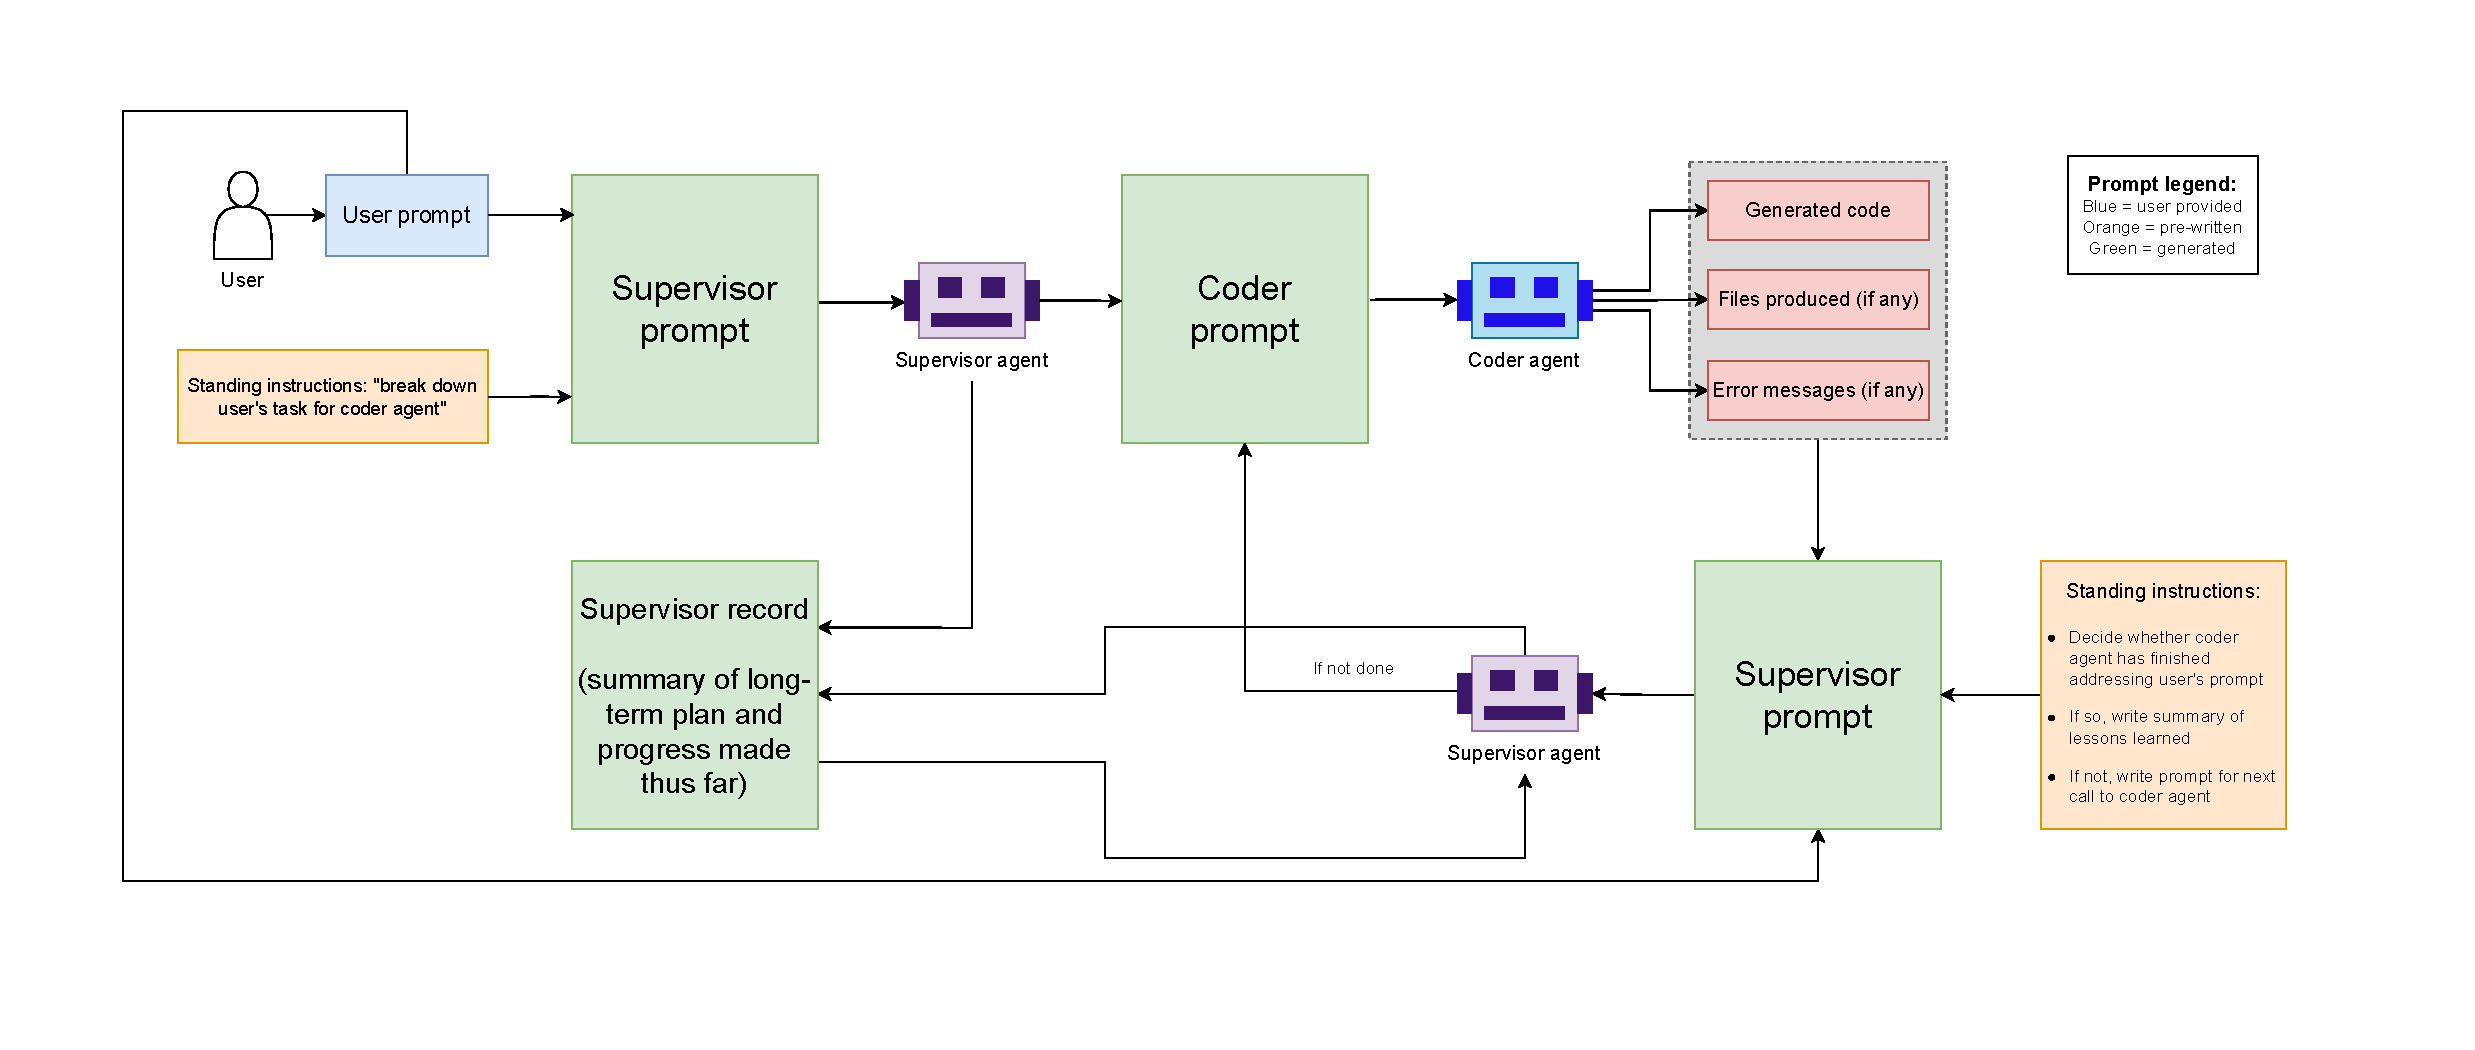
\includegraphics[width=0.95\textwidth]{supervisor_coder.pdf}
  \caption{
  \textbf{Illustration of the internal workflow for the supervisor–coder agent}. The blue box denotes user-provided prompts, orange boxes denote pre-written standing instructions (system prompts), and green boxes denote dynamically generated prompts created during the workflow. The supervisor decomposes the user’s task into subtasks, maintains an evolving supervisor record, and issues structured prompts to the coder agent. The coder returns generated code, intermediate files, and error messages, which the supervisor evaluates to determine whether the task has been completed or whether further refinement is required. This iterative supervisor–coder loop continues until the coder produces a valid solution or the maximum number of allowed attempts is reached.
}
  %\caption{Illustration of internal workflow for the supervisor–coder agent.}
  \label{fig:supervisor-coder-agent}
\end{figure*}

We design a supervisor-coder agent to carry out each task, as illustrated in Fig.~\ref{fig:supervisor-coder-agent}. The supervisor and coder are implemented as API calls to a LLM, with distinct system prompts tailored to their respective roles. The supervisor receives instructions from the human user, formulates corresponding directives for the coder, and reviews the coder’s output. The coder, in turn, takes the supervisor’s instructions and generates code to implement the required action. The generated code is executed through an execution engine, which records the execution trace. The supervisor and coder roles are defined by their differing access to state, memory, and system instructions. In the reference configuration, both roles are implemented using the \texttt{gemini-pro-2.5}~\cite{gemini_pro} model; however, the same architecture is applied to a range of contemporary LLMs to evaluate model-dependent performance and variability.
%In our tests, we use the \texttt{gemini-pro-2.5}~\cite{gemini_pro} model for both the supervisor and coder, though in principle any model could be used here.

% \begin{figure}
%   \centering
%   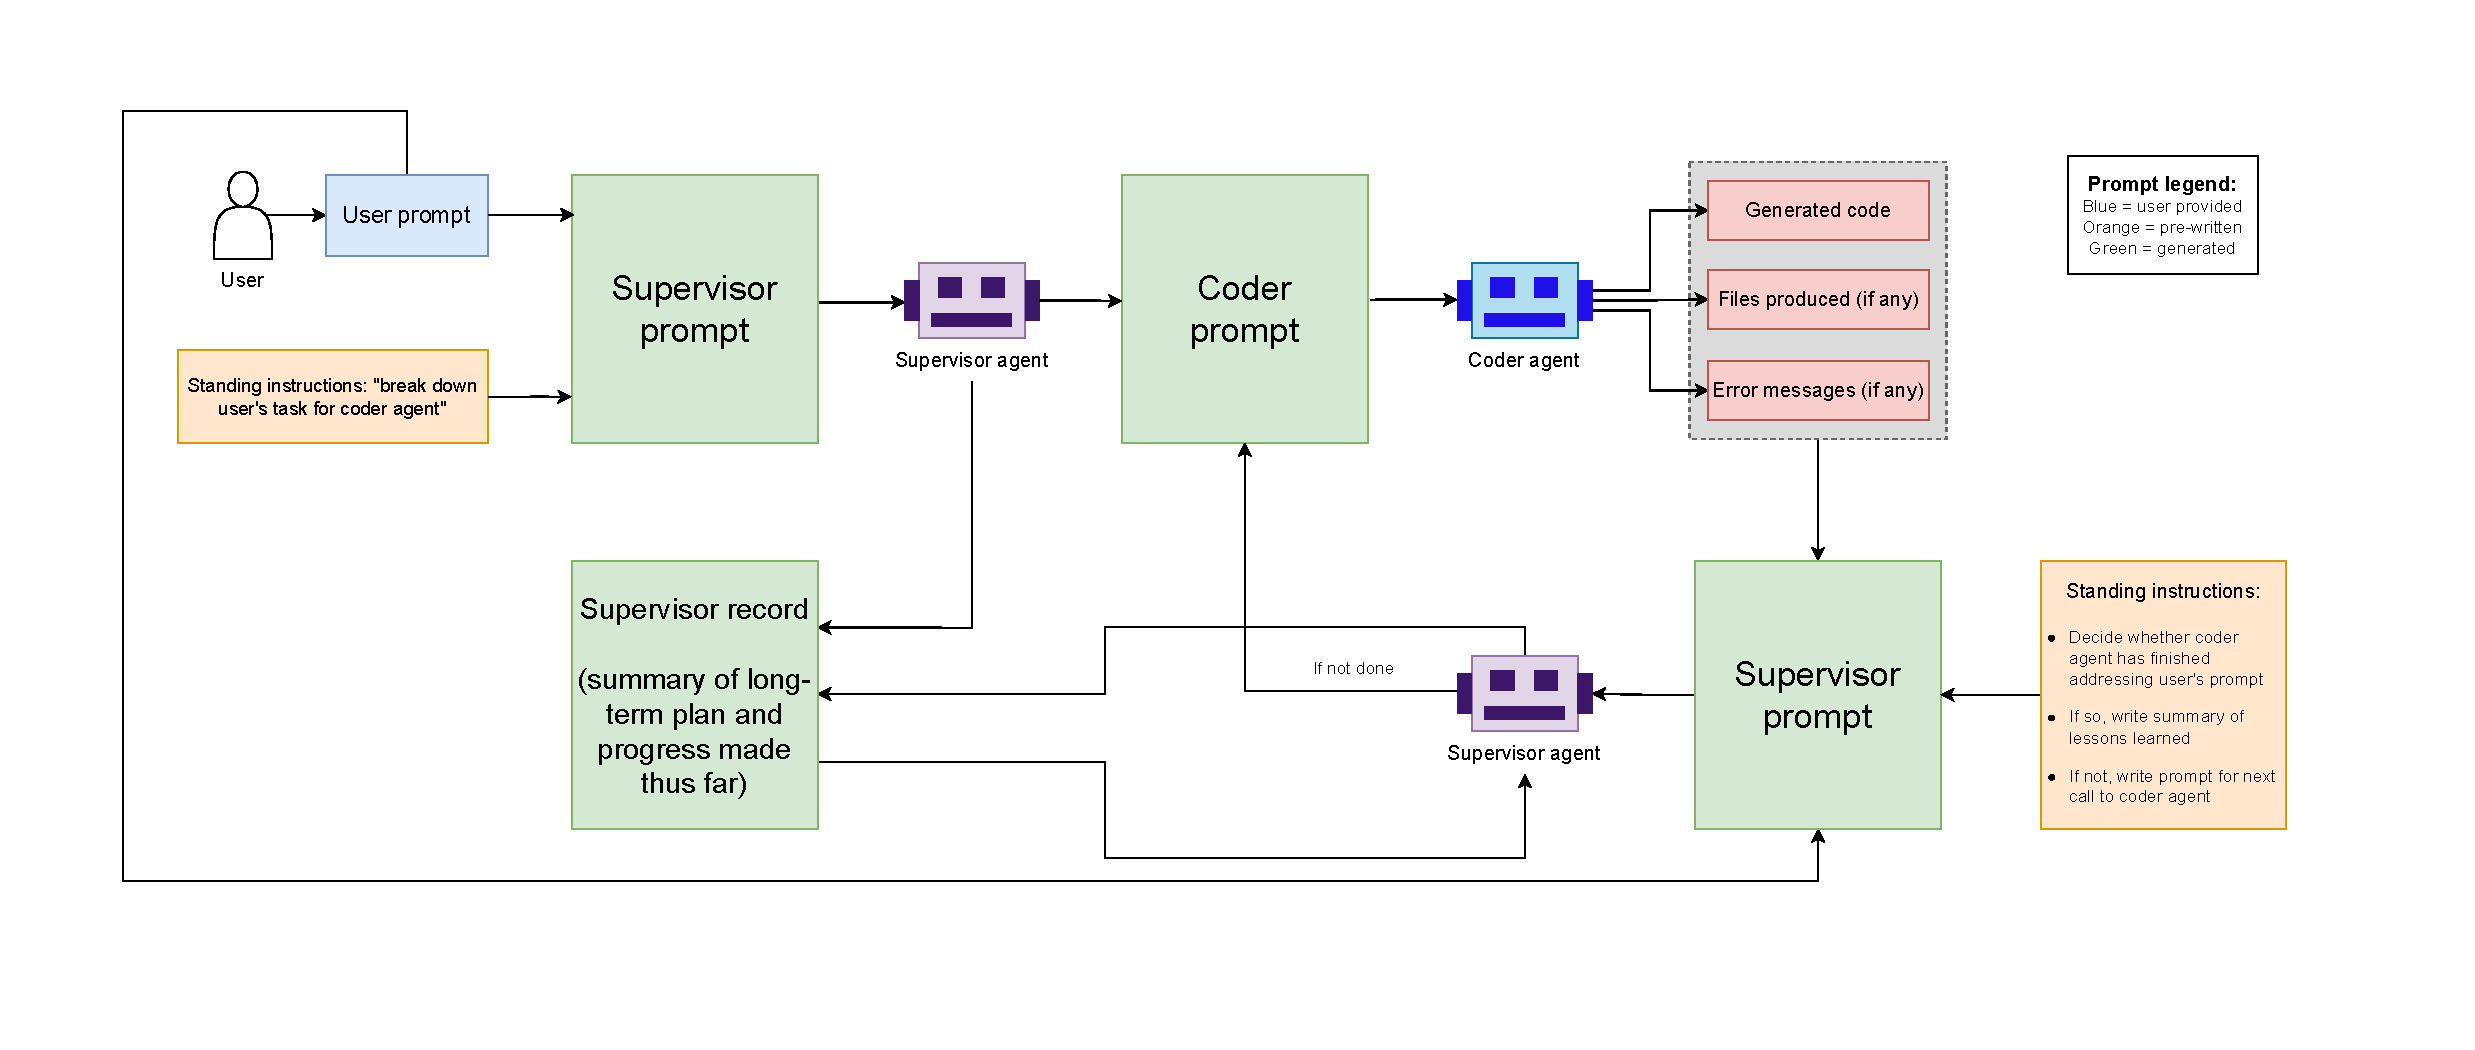
\includegraphics[width=0.9\linewidth]{supervisor_coder.pdf}
%   \caption{Illustration of internal workflow for the supervisor-coder agent.}\label{fig:supervisor-coder-agent}
% \end{figure}
Each agent interaction is executed through API calls to the LLM. Although we set the temperature to 0, other sampling parameters (e.g., top-p, top-k) remained at their default values, and some thinking-oriented models internally raise the effective temperature. As a result, the outputs exhibit minor stochastic variation even under identical inputs. Each call includes a user instruction, a system prompt, and auxiliary metadata for tracking errors and execution records.
%The supervisor and coder are implemented through API calls to the LLM. Each API call samples from the model’s probability distribution using the default inference settings of the respective API, including parameters such as temperature, top-p, and top-k, which were not modified from their default values. Consequently, the generated outputs exhibit a small degree of stochastic variation even under identical inputs. The input prompt to each API call consists of a user instruction, a system prompt, and auxiliary information for tracking errors and implementation records.

For the initial user interaction with the supervisor, the input prompt includes a natural-language description of the task objectives, suggested implementation strategies, and a system prompt that constrains the behavior of the model output. The result of this interaction is an instruction passed to the coder, which in turn generates a Python script to be executed. If execution produces an error, the error message, the original supervisor instruction, the generated code, and a debugging system prompt are passed back to the supervisor in a follow-up API call. The supervisor then issues revised instructions to the coder to address the problem. This self-correction loop is repeated up to three times, after which the trial is marked unsuccessful and the process stops.
%The supervisor and coder are implemented through API calls to the LLM. The temperature parameter, which controls the randomness of the generated output, was fixed to $0$ for all API calls to promote reproducibility. The input prompt to an API call typically consists of a user instruction, a system prompt, and auxiliary information for tracking errors and implementation records. For the initial user interaction with the supervisor, the input prompt includes a natural language description of the task objectives, suggested implementation strategies, and a system prompt that guides the behavior of the LLM output. The output of this user–supervisor interaction is an instruction passed to the coder, based on which the coder generates a Python script to be executed. If execution results in an error, the error message, the original supervisor instruction, the generated code, and a debugging system prompt are passed back to the supervisor via another API call. The supervisor then produces revised instructions for the coder to address the errors. This self-correction process is allowed up to five times before the trial is deemed unsuccessful.

  % \item \textbf{Inference time.} We used a third-party API call provider that routes our requests to different cloud computing providers hosting a variety of models. The finite LLM inference time introduces latency in the workflow, making it important to assess inference time for task completion. However, due to uncertainties and variable conditions in networking and API routing, we report only the order of magnitude of inference time as a sanity check.  

\section{Results}
\subsection{Statistics-enriched}
To establish a baseline, we conducted 219 experiments with the \texttt{gemini-pro-2.5} model, providing high statistical precision across all analysis stages. In this configuration, the workflow was organized into three composite steps: (1) \textbf{data preparation}, including \textit{ROOT file inspection}, \textit{ntuple conversion}, and \textit{preprocessing}; (2) \textbf{signal-background (S-B) separation}; and (3) \textbf{categorization} based on the expected Higgs-to-diphoton significance. Up to five self-correction iterations were permitted, as preliminary experiments showed that additional attempts rarely improved outcomes while incurring significantly higher computational cost. The corresponding success rates for these three steps were 58~$\pm$ 3\%, 88~$\pm$ 2\%, and 74~$\pm$ 3\%, respectively.
%To establish a baseline, we conducted 219 experiments with the \texttt{gemini-pro-2.5} model, providing high statistical precision across all analysis stages. In this configuration, the workflow was organized into three composite steps: (1) \textbf{data-preparation} including \textit{ROOT file inspection}, \textit{ntuple conversion}, and \textit{preprocessing}; (2) \textbf{signal–background (S-B) separation}; and (3) \textbf{categorization} based on the expected Higgs-to-photon significance. Up to five self-corrections were permitted, as preliminary experiments showed that additional attempts rarely improved outcomes while incurring higher computational cost. The corresponding success rates for these three steps were 58 $\pm$ 3\%, 88 $\pm$ 2\%, and 74 $\pm$ 3\%, respectively.

\begin{table}[htbp]
\centering
\resizebox{\linewidth}{!}{%
\begin{tabular}{l S[table-format=3.0] S[table-format=3.0] S[table-format=3.0]}
\hline
\textbf{Error type} & \textbf{Data-prep} & \textbf{S--B sep.} & \textbf{Categorization} \\
\hline\hline
All data weights = 0        & 41 & 0  & 0  \\
Dummy data created          & 15 & 4  & 4  \\
Function-calling error      & 1  & 3  & 26 \\
Incorrect branch name       & 9  & 0  & 0  \\
Intermediate file not found & 17 & 13 & 6  \\
Semantic error              & 6  & 5  & 17 \\
Other                       & 4  & 0  & 4  \\
\hline
\textbf{Total failures}     & \textbf{93} & \textbf{25} & \textbf{57} \\
\hline
\end{tabular}
} % end resizebox

\vspace{6pt}
\caption{
Distribution of failure counts by error category across the three workflow stages, based on 219 trials per step. Each row lists the number of failures attributable to a given error type; the bottom row reports the total failures per stage.
}
\label{tab:error_types}
\end{table}
To analyze failure modes, we examined the model-generated log files for all unsuccessful trials and grouped recurrent issues into seven error categories. These categories correspond to the most frequently observed patterns across the logs and reflect dominant failure modes in agent-driven HEP workflows. As summarized in Table~\ref{tab:error_types}, the \textbf{data-preparation} (data-prep) stage was the most error-prone, with 93 failures out of 219 trials. Most issues arose from insufficient context for identifying objects within \textsc{ROOT} files. The most common error types - \textit{all data weights = 0} and \textit{intermediate file not found} - indicate persistent challenges in reasoning about file structures, dependencies, and runtime organization. Providing richer execution context, such as package lists, file hierarchies, and metadata, may help mitigate these problems. Despite these limitations, the overall completion rate ($\sim$57\%) demonstrates that LLMs can autonomously execute complex domain-specific programming tasks a nontrivial fraction of the time.
%As summarized in Table \ref{tab:error_types}, the \textbf{data-preparation} stage was the most error-prone, with 93 failures out of 219 trials. Most issues stemmed from insufficient context for identifying objects within \textsc{ROOT} files. The dominant failure modes were Type 1 (zero event weights) and Type 5 (missing intermediate files), indicating persistent challenges in reasoning about file structures, dependencies, and runtime organization. Providing richer execution context such as package lists, file hierarchies, and metadata could help mitigate these problems. Despite these limitations, the overall completion rate ($\sim$ 57\%) demonstrates that LLMs can autonomously execute complex domain-specific programming tasks a non-trivial fraction of the time.

The subsequent \textbf{S–B separation} (S--B sep.) and \textbf{categorization} stages exhibited substantially fewer failures (25 and 57, respectively). In the S--B sep. step, the most common issue was \textit{intermediate file not found}, indicating that the agent occasionally lost track of file paths or dependencies across iterations. Once the workflow progressed to the \textbf{categorization} stage, failures were instead dominated by \textit{function-calling errors} and \textit{semantic errors}. This shift reflects the increased complexity of the categorization logic: the agent must iteratively construct valid function calls, interpret model outputs, and reason about numerical optimization criteria. These operations rely more heavily on precise syntax and conceptual understanding, making them more susceptible to calling and semantic mistakes despite the greater overall stability of later stages.
%The subsequent \textbf{S-B separation} using \texttt{TabPFN} and the final \textbf{categorization} for the Higgs-to-diphoton measurement exhibited substantially fewer failures (25 and 57, respectively). These errors were primarily Type 3 (function-calling) and Type 6 (semantic) issues, reflecting improved stability once the workflow reaches the model-training and evaluation stages.

To assess agent efficiency, we measured the ratio of user-input tokens to the total tokens exchanged with the API. For the \texttt{gemini-pro-2.5} baseline, this ratio was (1.65~$\pm$0.15)$\times 10^{-3}$ for \textbf{data preparation}, (1.43$\pm$0.10)$\times 10^{-3}$ for \textbf{S–B separation}, and (0.93$\pm$~0.07)$\times 10^{-3}$ for \textbf{categorization}. A higher ratio indicates more efficient task execution, as fewer internally generated tokens are required to complete the same instruction set. Over 98\% of tokens originated from the model’s autonomous reasoning and self-correction rather than direct user input, suggesting that providing additional prompt detail would minimally affect overall token cost. This ratio therefore serves as a simple diagnostic of communication efficiency and reasoning compactness.
%To assess agent efficiency, we measured the ratio of user-input tokens to the total tokens exchanged with the API. For the \texttt{gemini-pro-2.5} baseline, this ratio was (1.65 $\pm$ 0.15) $\times$ $10^{-3}$ for \textbf{data preparation}, (1.43 $\pm$ 0.10) $\times$ $10^{-3}$ for \textbf{S-B separation}, and (0.93 $\pm$ 0.07) $\times$ $10^{-3}$ for \textbf{categorization}. A higher ratio indicates more efficient task execution, as fewer internally generated tokens are required to complete the same instruction set. Over 98\% of tokens originated from the model’s autonomous reasoning and self-correction rather than direct user input, suggesting that additional task detail would minimally affect overall token cost. This ratio thus provides a simple diagnostic of communication efficiency and reasoning compactness.

\subsection{LLM benchmarks}
\begin{figure*}[htbp]
  \centering

  % --- (a) Success Rate ---
  \begin{subfigure}{0.7\textwidth}   % SAME WIDTH
    \hspace{-3.0cm}
    \centering
    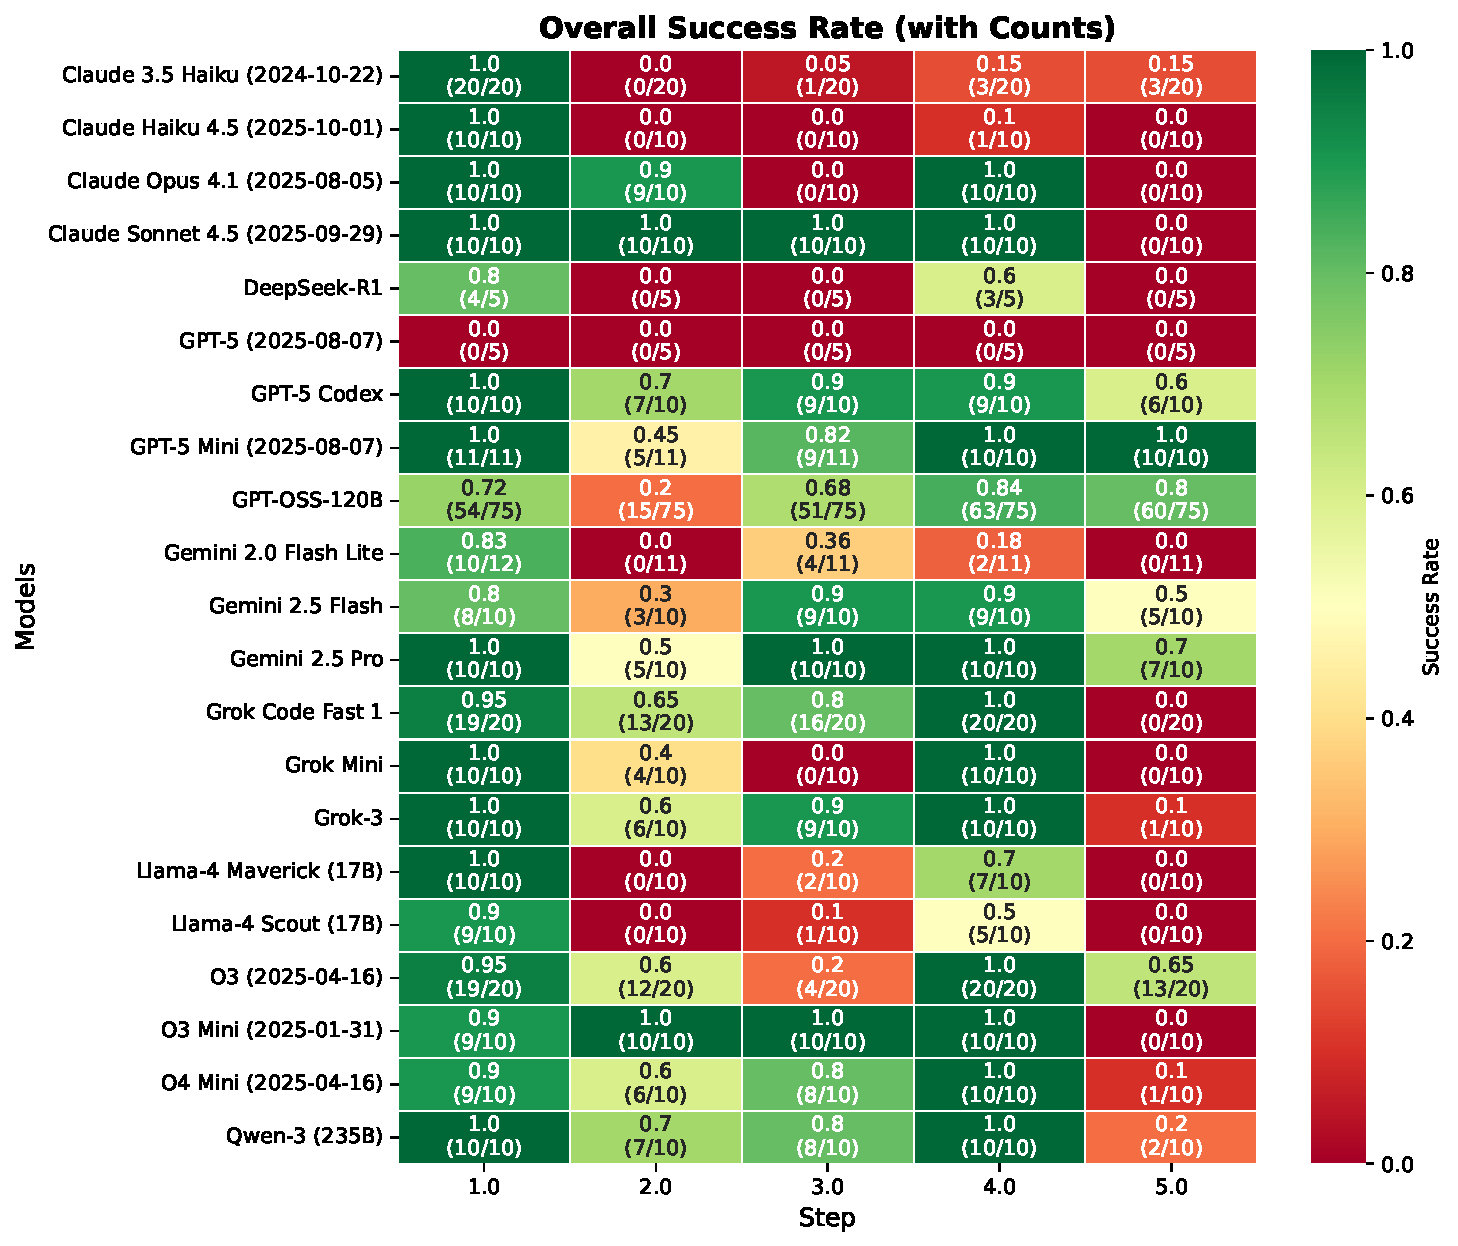
\includegraphics[width=\textwidth]{1_success_rate_heatmap.pdf}
    \caption{Success rate}
    \label{fig:success_heatmap}
  \end{subfigure}

  \vspace{1.2em}

  % --- (b) Error Distribution ---
  \begin{subfigure}{0.75\textwidth}   % SAME WIDTH
    \centering
    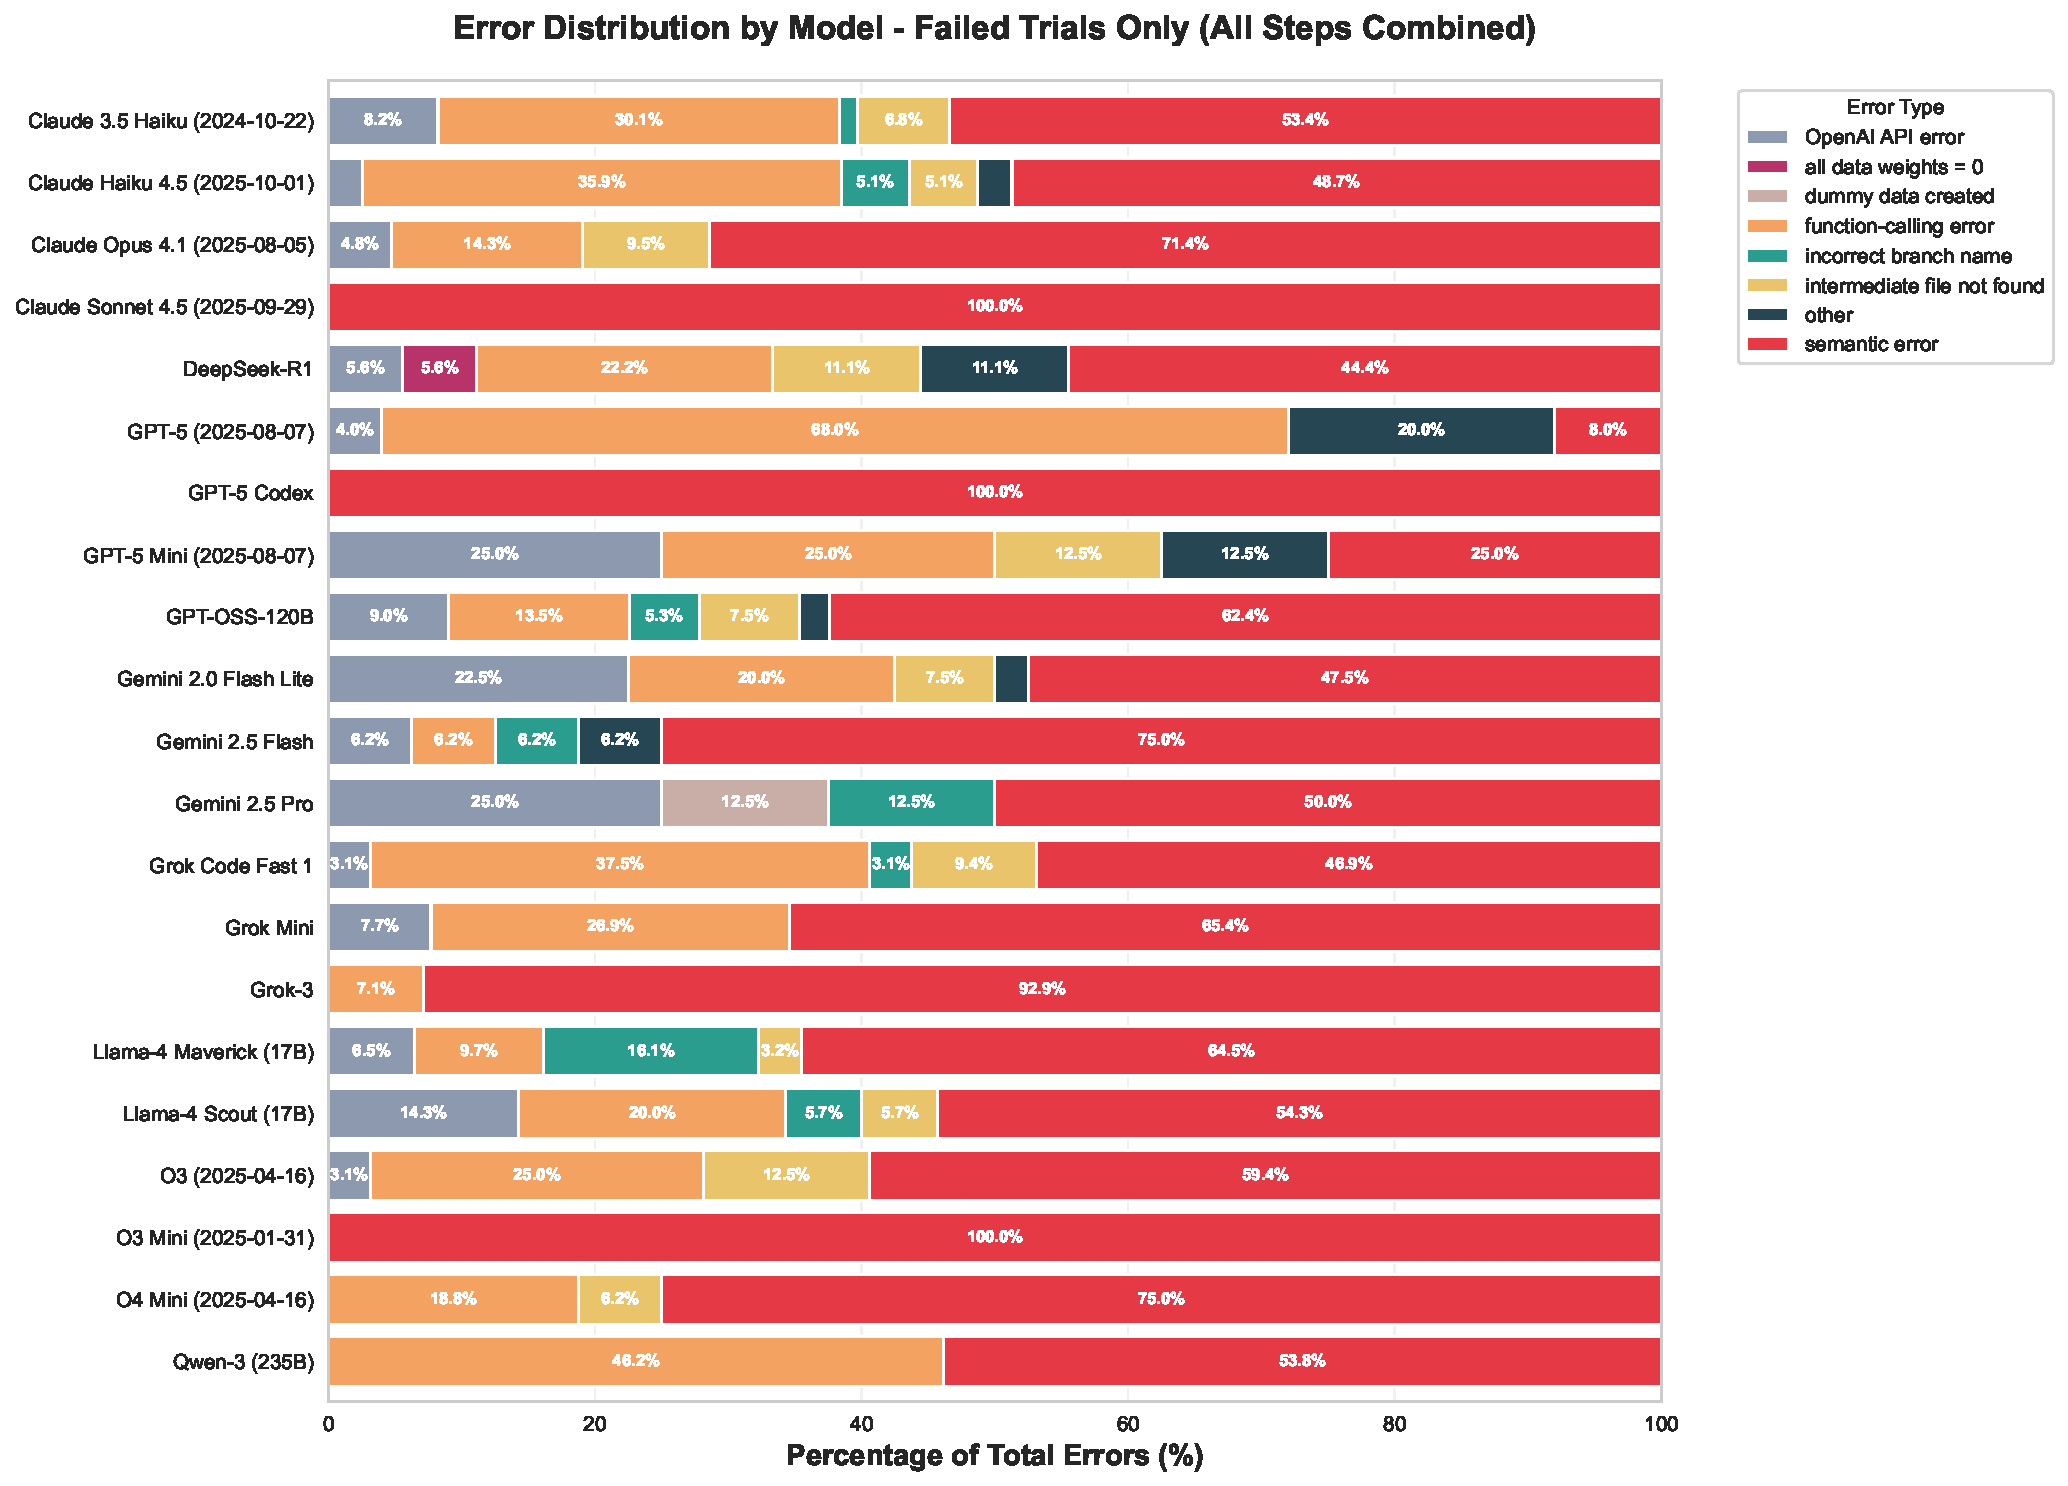
\includegraphics[width=\textwidth]{error_distribution_by_model.pdf}
    \caption{Error distribution}
    \label{fig:error_distribution}
  \end{subfigure}

  \caption{
    Cross-model comparison of LLM-agent performance.
    (a) Success fraction for each model-step pair.
    (b) Error distribution across all failed trials for each model.
  }
  \label{fig:model_comparison}
\end{figure*}
% \begin{figure*}[htbp]
%   \centering

%   \begin{minipage}{\textwidth}
%     \centering

%     % --- (a) ---
%     \begin{subfigure}[t]{0.44\textwidth}
%       \centering
%       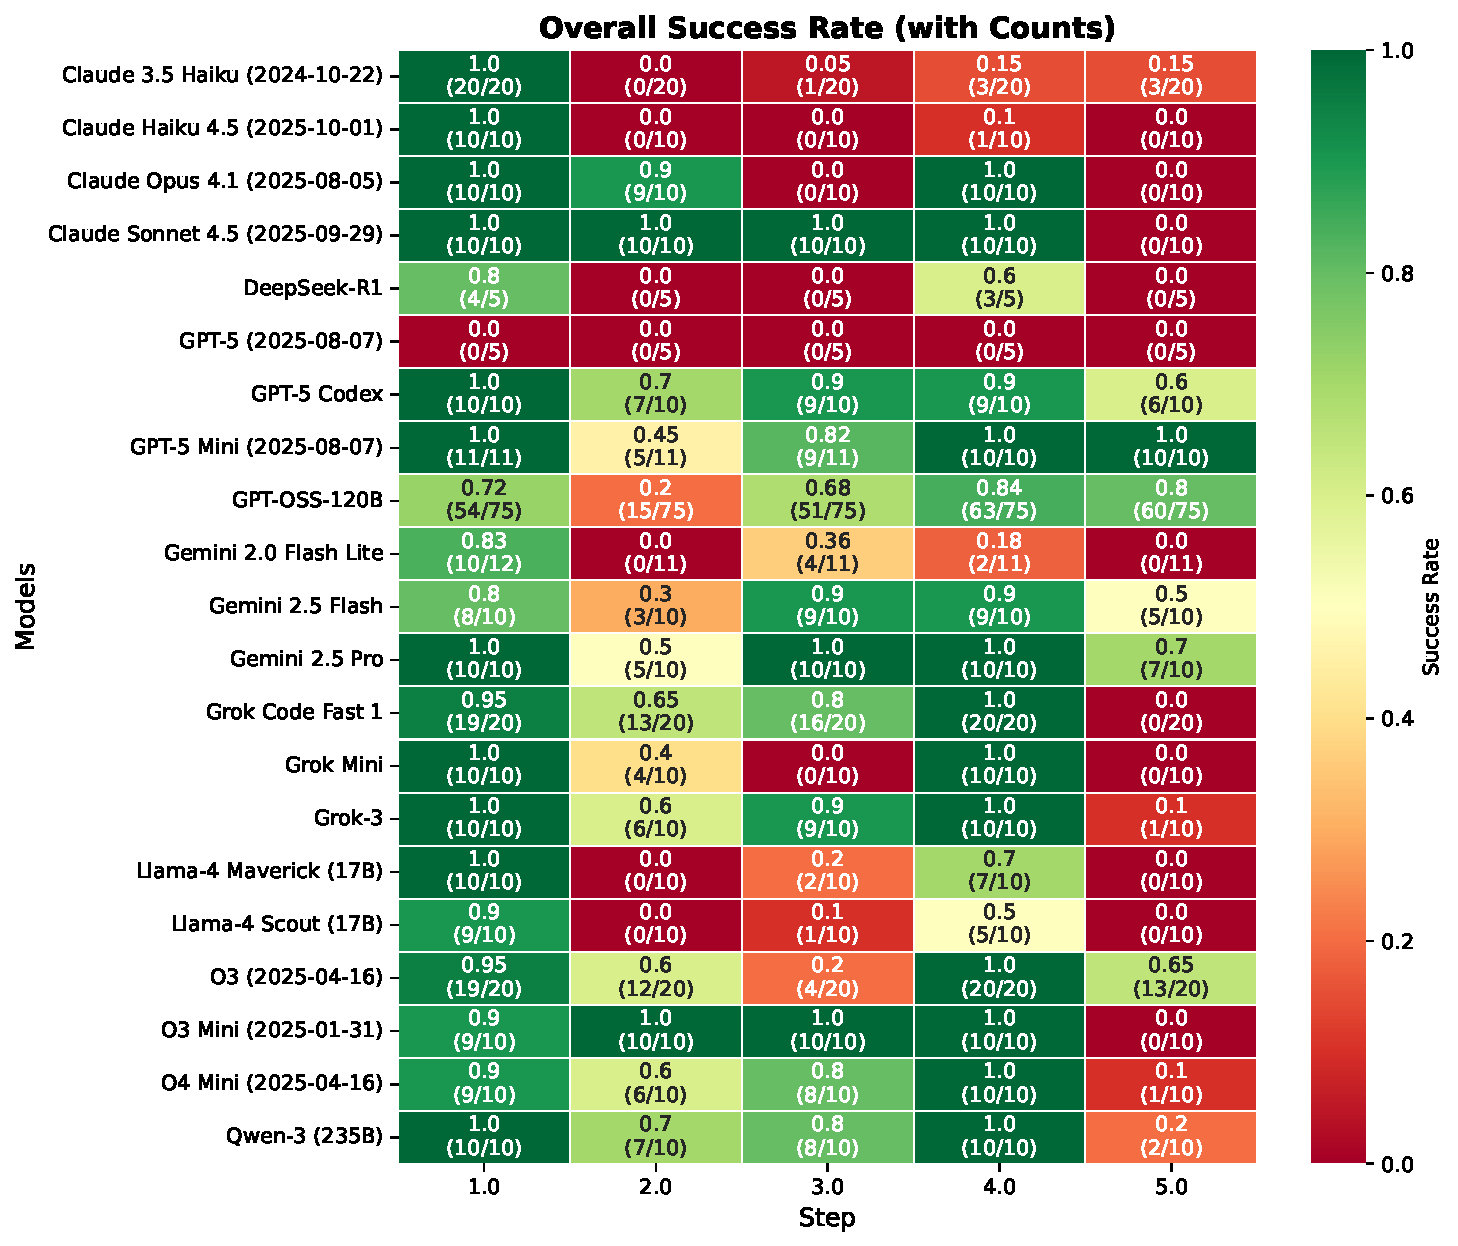
\includegraphics[width=\textwidth]{1_success_rate_heatmap.pdf}
%       \caption{Success rate}
%       \label{fig:success_heatmap}
%     \end{subfigure}
%     \hfill
%     % --- (b) ---
%     \begin{subfigure}[t]{0.54\textwidth}
%       \centering
%       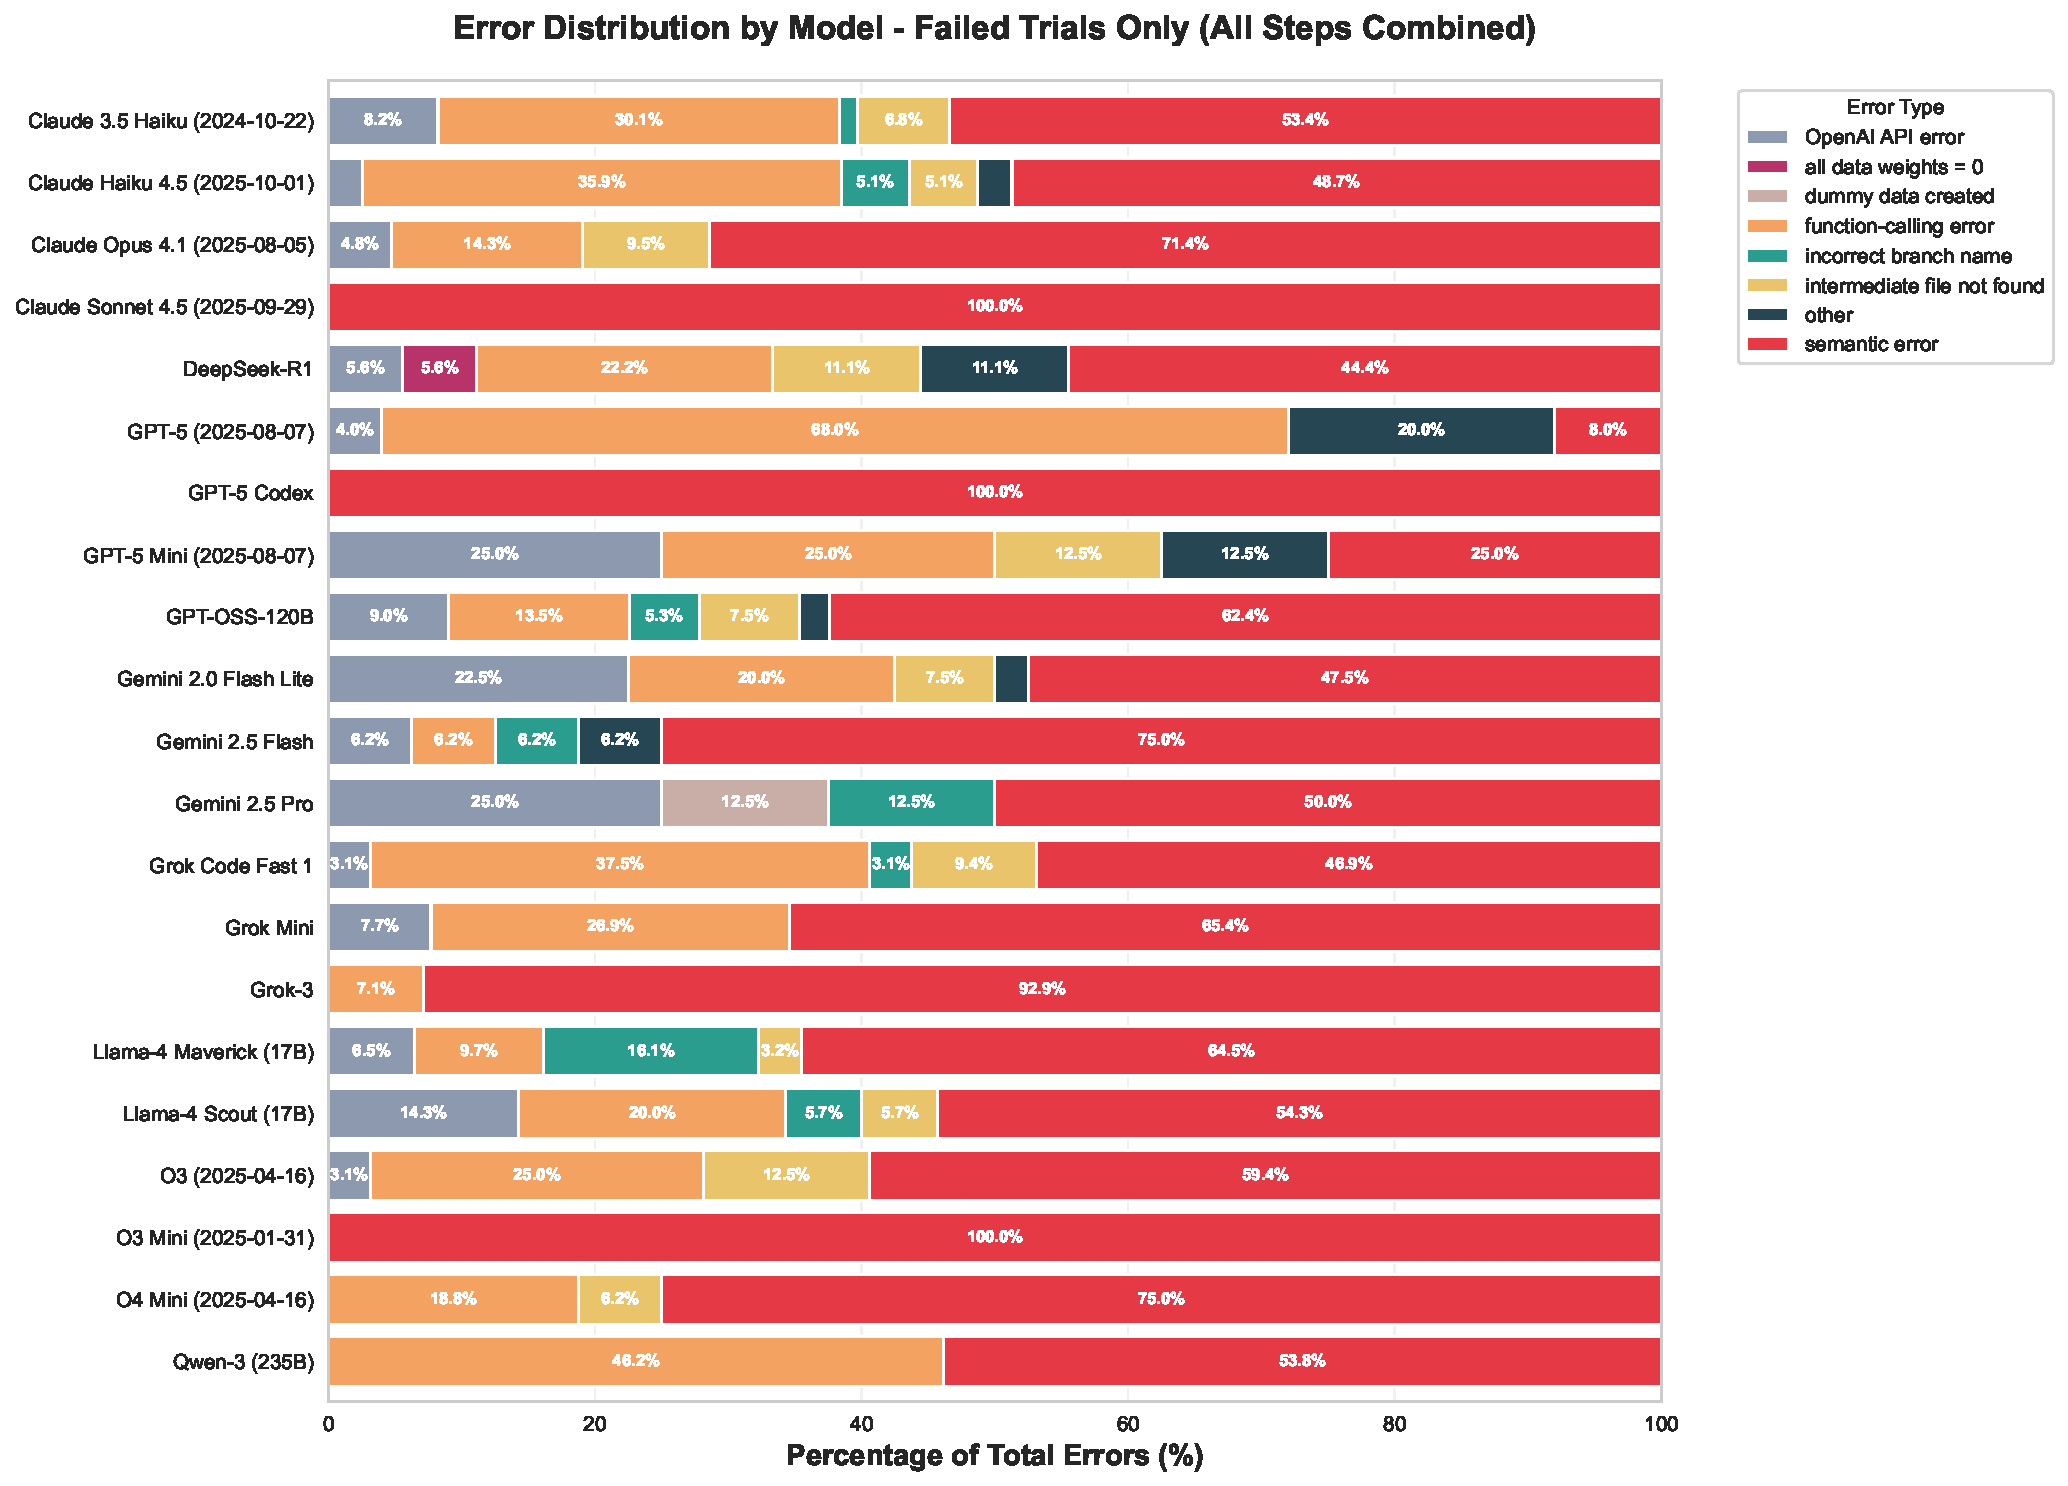
\includegraphics[width=\textwidth]{error_distribution_by_model.pdf}
%       \caption{Error distribution}
%       \label{fig:error_distribution}
%     \end{subfigure}

%   \end{minipage}

%   \vspace{6pt}

%   \caption{
%     Cross-model comparison of LLM-agent performance.
%     (a) Success fraction for each model-step pair.
%     (b) Distribution of error magnitudes by model, summarizing the variability and characteristic failure patterns across models. Bars without numerical labels correspond to fractions below 3\%, omitted for clarity. }
%   \label{fig:model_comparison}
% \end{figure*}
Following the initial benchmark with \texttt{gemini-pro-2.5}, we expanded the study to include additional models, such as \texttt{openai-gpt-5}~\citep{gpt5}, \texttt{claude-3.5}~\citep{anthropic2024claude35}, \texttt{qwen-3}~\citep{qwen3}, and the open-weight \texttt{gpt-oss-120b}~\citep{openai2025gptoss120bgptoss20bmodel}, evaluated under the same agentic workflow. Based on early observations, the prompt for the \textbf{data-preparation} stage was refined and subdivided into three subtasks: \textbf{ROOT file inspection}, \textbf{ntuple conversion}, and \textbf{preprocessing} (including signal and background region selection), as described in Section~\ref{sec:description_HEP_analysis}. Input file locations were also made explicit for an agent to ensure deterministic resolution of data paths and reduce reliance on implicit context.

The results across models, summarized in Figs.~\ref{fig:success_heatmap}–\ref{fig:error_distribution}, show consistent qualitative behavior with the baseline while highlighting quantitative differences in reliability, efficiency, and error patterns. For the \texttt{gemini-pro-2.5} model, the large number of repeated trials (219 total) provides a statistically robust characterization of performance across steps. For the other models - each tested with approximately ten trials per step - the smaller sample size limits statistical interpretation, and the results should therefore be regarded as qualitative indicators of behavior rather than precise performance estimates. Nonetheless, the observed cross-model consistency and similar failure patterns suggest that the workflow and evaluation metrics are sufficiently general to support larger-scale future benchmarks. This pilot-level comparison thus establishes both the feasibility and reproducibility of the agentic workflow across distinct LLM architectures.

Figure~\ref{fig:success_heatmap} summarizes the cross-model performance of the agentic workflow. The heatmap shows the success rate for each model–step pair, highlighting substantial variation in reliability across architectures. The dates appended to each model name denote the model release or update version used for testing, while the parameter in parentheses (e.g., ``17B'') indicates the model’s approximate parameter count in billions. Models in the \texttt{GPT-5} and \texttt{Gemini} families achieve the highest completion fractions across most steps, whereas smaller or open-weight models such as \texttt{gpt-oss-120b} exhibit lower but still non-negligible success on certain steps.
This demonstrates that the workflow can be executed end-to-end by multiple LLMs, though with markedly different robustness and learning stability.

\subsection{LLM-Driven Error Analysis}
Figure \ref{fig:error_distribution} shows the distribution of failure modes across all analysis stages, considering only trials that did not reach a successful completion. The categorization is based on the LLM-generated outputs themselves, capturing how each model typically fails. Error types include function-calling issues, missing or placeholder data, infrastructure problems (e.g., API or file-handling failures), and semantic errors - cases where the model misinterprets the prompt and produces runnable but incorrect code, as well as syntax mistakes.

During each run of the LLM agent workflow, two complementary log files are generated to assist in analysing and categorizing errors. An example of each log file can be found in Appendix \ref{appendix:log_files_and_error_analysis}.
\begin{itemize}
    \item \textbf{Comprehensive Log:} This file captures all LLM inputs and outputs across every call, as well as coder execution results.
    \item \textbf{Validation Log:} Here, the outputs produced by the LLM are compared against reference solutions, marked as failures if there are any structural mismatches (e.g., shape or dimension differences in numpy arrays) or content disparities. Outputs must match the solution exactly to pass. 
\end{itemize}

These log files serve as direct input for our LLM-based error classification pipeline. 

Error classification in our workflow is performed by a dedicated LLM (\texttt{gpt-oss-120b}), guided by a carefully engineered prompt to ensure standardized and unambiguous categorization. The prompt construction follows these principles:

\begin{itemize}
    \item \textbf{Agent Role:} The model is explicitly instructed to act as an expert on artificial intelligence workflow failures in high energy physics.
    \item \textbf{Workflow Summary:} The prompt summarizes the supervisor/coder workflow:
    \begin{itemize}
        \item The user provides an analysis prompt.
        \item A supervisor agent decomposes the task and instructs a coder agent.
        \item The coder agent generates code, which is then executed.
        \item The supervisor reviews execution outcomes and iterates with the coder as needed until completion.
    \end{itemize}
    \item \textbf{Error Categories:} The LLM receives the following list of possible error categories:
    \begin{itemize}
        \item \texttt{all data weights = 0}
        \item \texttt{dummy data created}
        \item \texttt{function-calling error}
        \item \texttt{incorrect branch name}
        \item \texttt{intermediate file not found}
        \item \texttt{semantic error}
        \item \texttt{other}
    \end{itemize}
    \item \textbf{Task Definition:} The prompt directs the model to select the \emph{single most appropriate} error category for each case, prioritizing root causes over superficial error messages. This means the categorization targets fundamental issues, such as logic mistakes, missing dependencies, data mismatches, or miscommunications. 
    \item \textbf{Strict Output Structure:} The model must return only the category name, wrapped in triple asterisks (e.g. \verb|***Category***|), with no additional explanation or content. This requirement allows for robust and automated parsing of the outputs.
    \item \textbf{Log File Inclusion:} Both the comprehensive and validation logs are provided to the LLM for context, ensuring informed and accurate error classification.
\end{itemize}

This prompt design ensures reproducible and interpretable error analysis, allowing us to systematically quantify and address failure modes within LLM-driven analysis workflows. 

Clear model-dependent patterns emerge. Models with higher success rates, such as the \texttt{GPT-5} and \texttt{Gemini 2.5} families, show fewer logic and syntax issues, while smaller or open-weight models exhibit more semantic and data-handling failures. These differences reveal characteristic failure signatures that complement overall completion rates. 
%Figure \ref{fig:error_distribution} summarizes the distribution of failure modes aggregated across all analysis steps.  Each bar represents the normalized composition of errors for a given model, grouped into categories such as function-calling errors, missing or dummy data generation, semantic errors, and infrastructure issues (e.g., API or file-handling failures). The resulting patterns highlight substantial model-dependent variability: models with high success rates, such as those in the \texttt{GPT-5} and \texttt{Gemini 2.5} families, exhibit a smaller fraction of logic- or syntax-related failures, whereas smaller or open-weight models show a larger share of semantic and data-handling mistakes.  These trends indicate that even when overall completion rates are comparable, the qualitative nature of errors differs systematically across architectures, providing complementary insight into model robustness and the underlying failure mechanisms of agentic workflows.

Taken together, Figure~\ref{fig:model_comparison} highlights two main aspects of LLM-agent behavior: overall task reliability and the characteristic error modes behind failed executions. These results show that models differ not only in success rate but also in the nature of their failures, providing insight into their robustness and limitations in realistic HEP workflows.
%Taken together, Figure~\ref{fig:model_comparison} highlights two key aspects of LLM-agent behavior in this workflow: (i) task reliability across architectures, and (ii) the characteristic error modes underlying incomplete executions. These results provide a practical basis for comparing models not only by their aggregate success rate, but also by the qualitative nature of their failures, offering insight into robustness and model-specific limitations in realistic HEP analysis pipelines.
% Taken together, Figure~\ref{fig:model_comparison} demonstrates three key aspects of LLM-agent behavior in this workflow: (i) task reliability across architectures, (ii) the degree of autonomous effort needed for successful execution, and (iii) the associated computational and financial cost. These results provide a practical basis for comparing models not only on success rate, but also on their efficiency and operational viability in realistic high energy physics analysis pipelines.
\begin{figure*}[htbp]
  \centering
  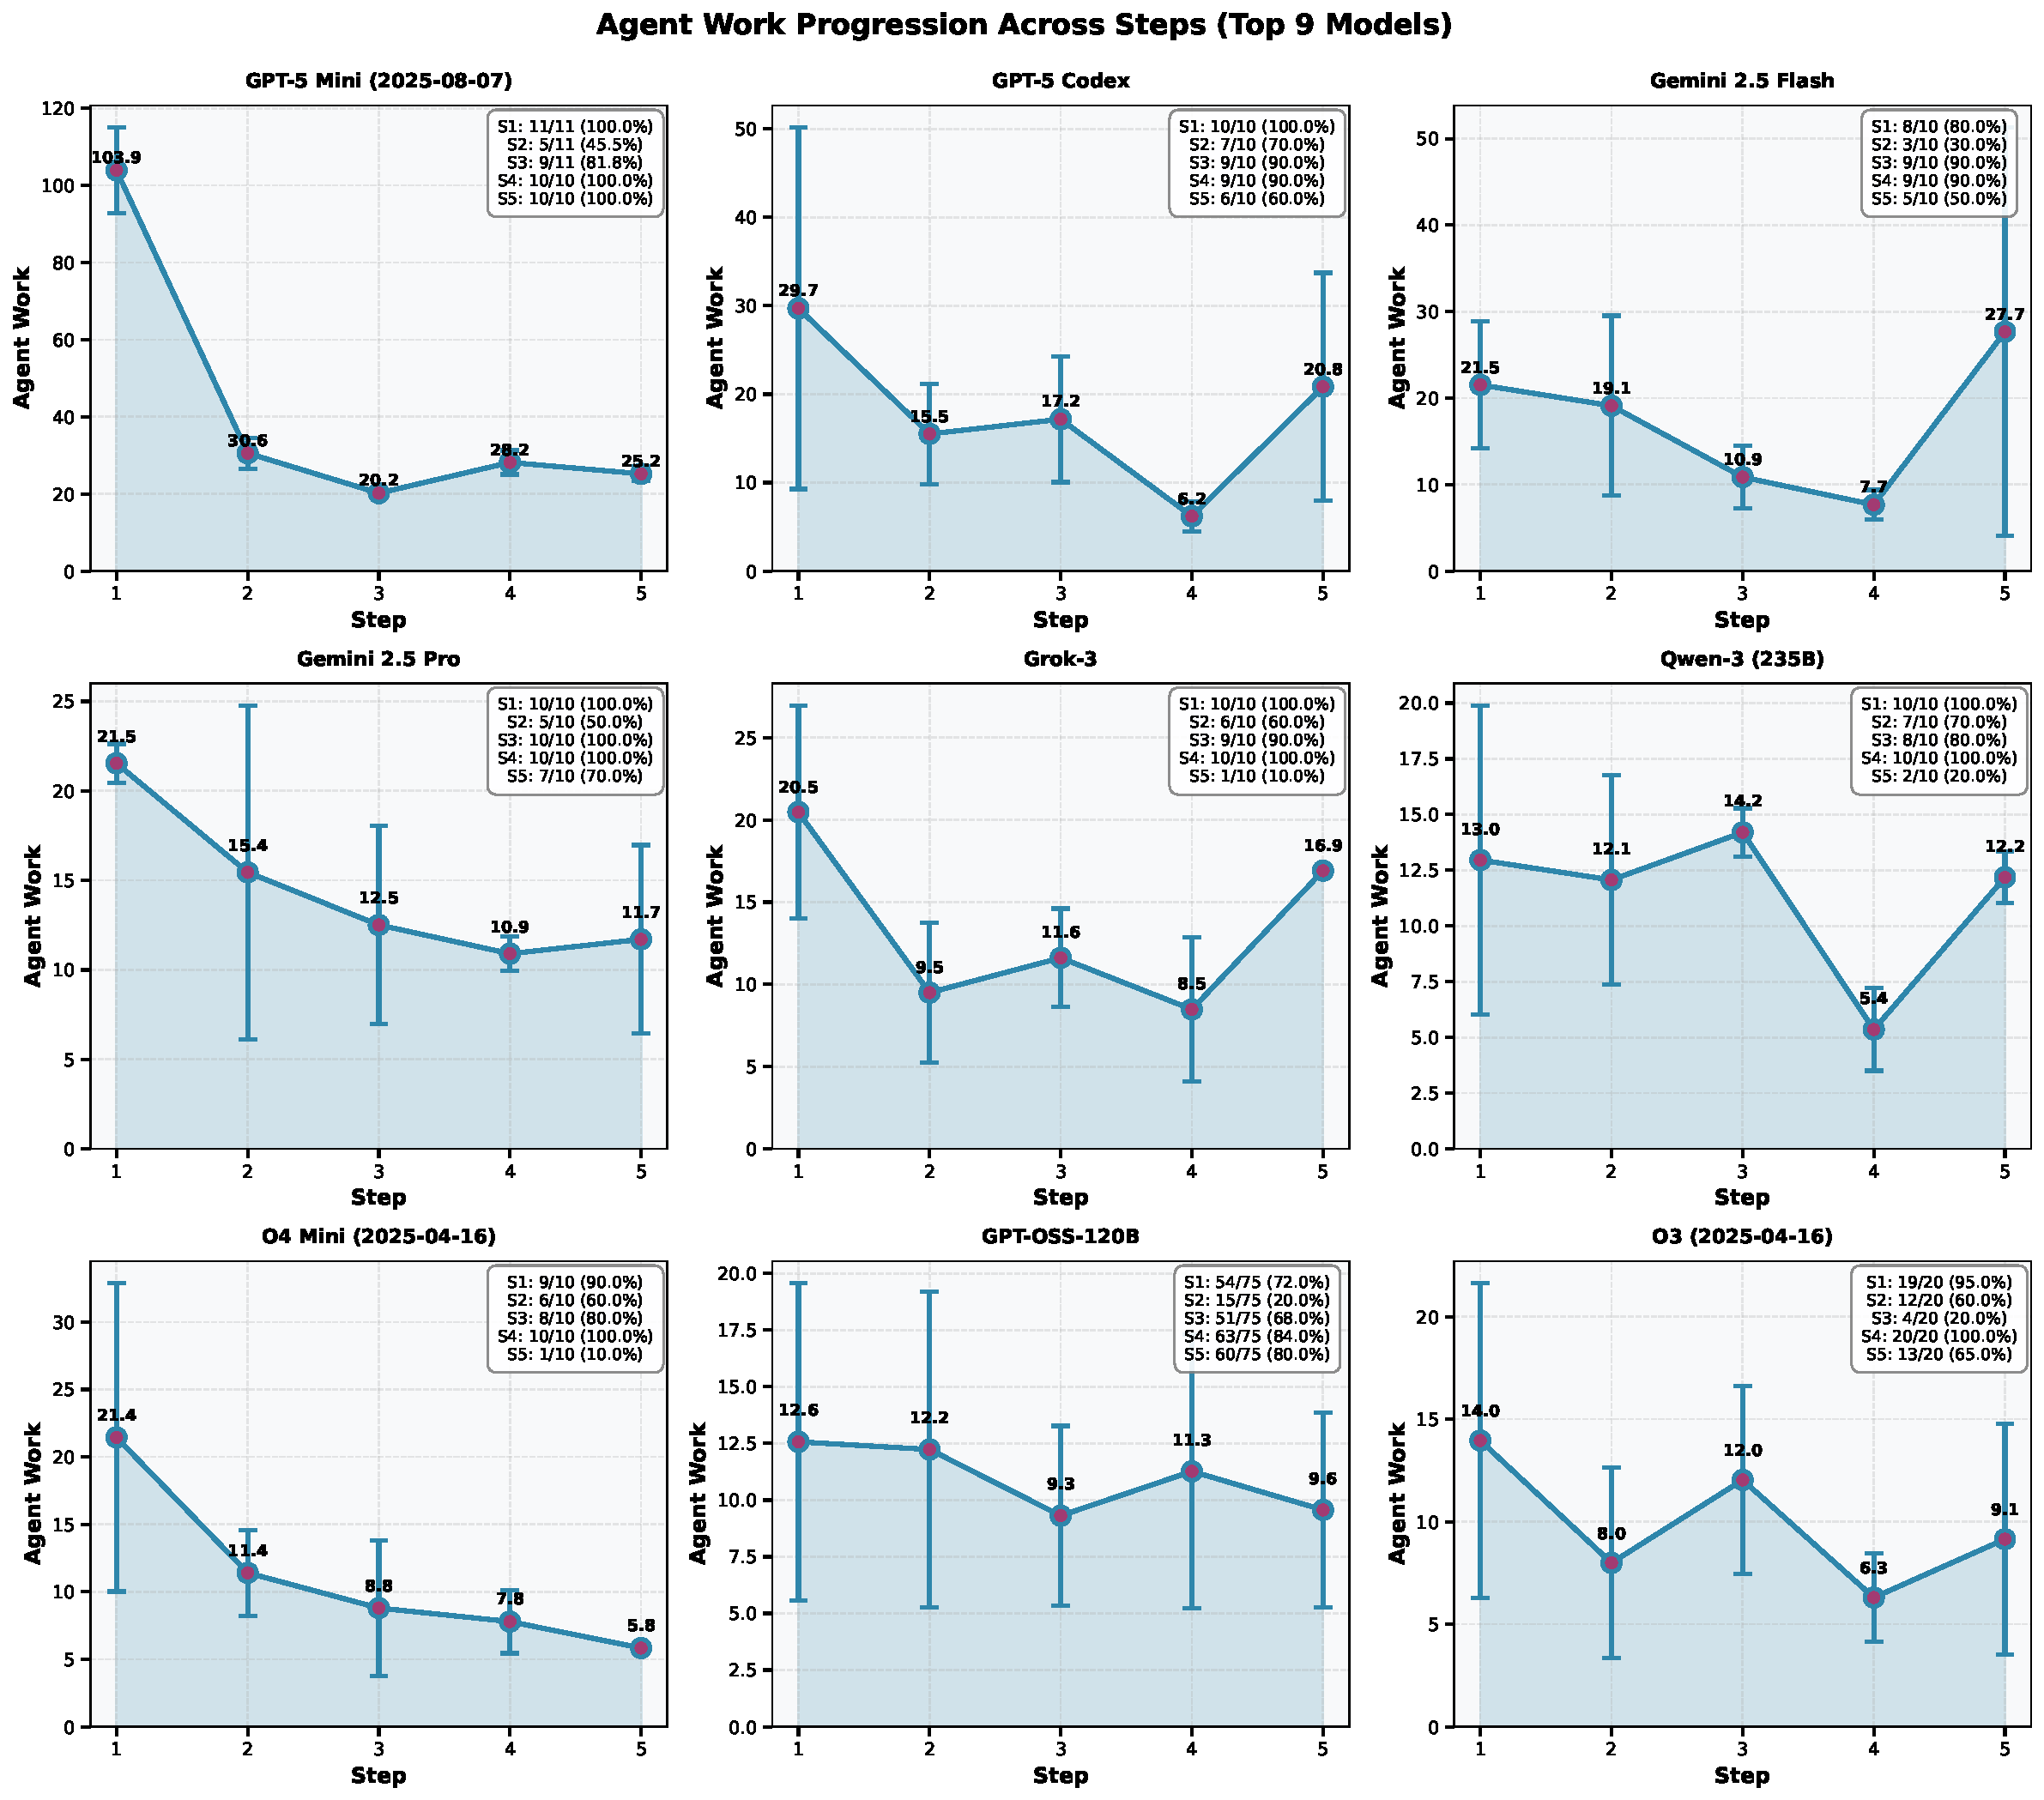
\includegraphics[width=0.95\textwidth]{2_agent_work_line_plot.pdf}
  \caption{
    \textbf{Agent work progression across workflow steps.}
    Average agent work (with standard-deviation error bars) shown for the nine
    models that successfully completed all stages of the workflow.
  }
  \label{fig:agent_work}
\end{figure*}

\begin{figure*}[htbp]
  \centering
  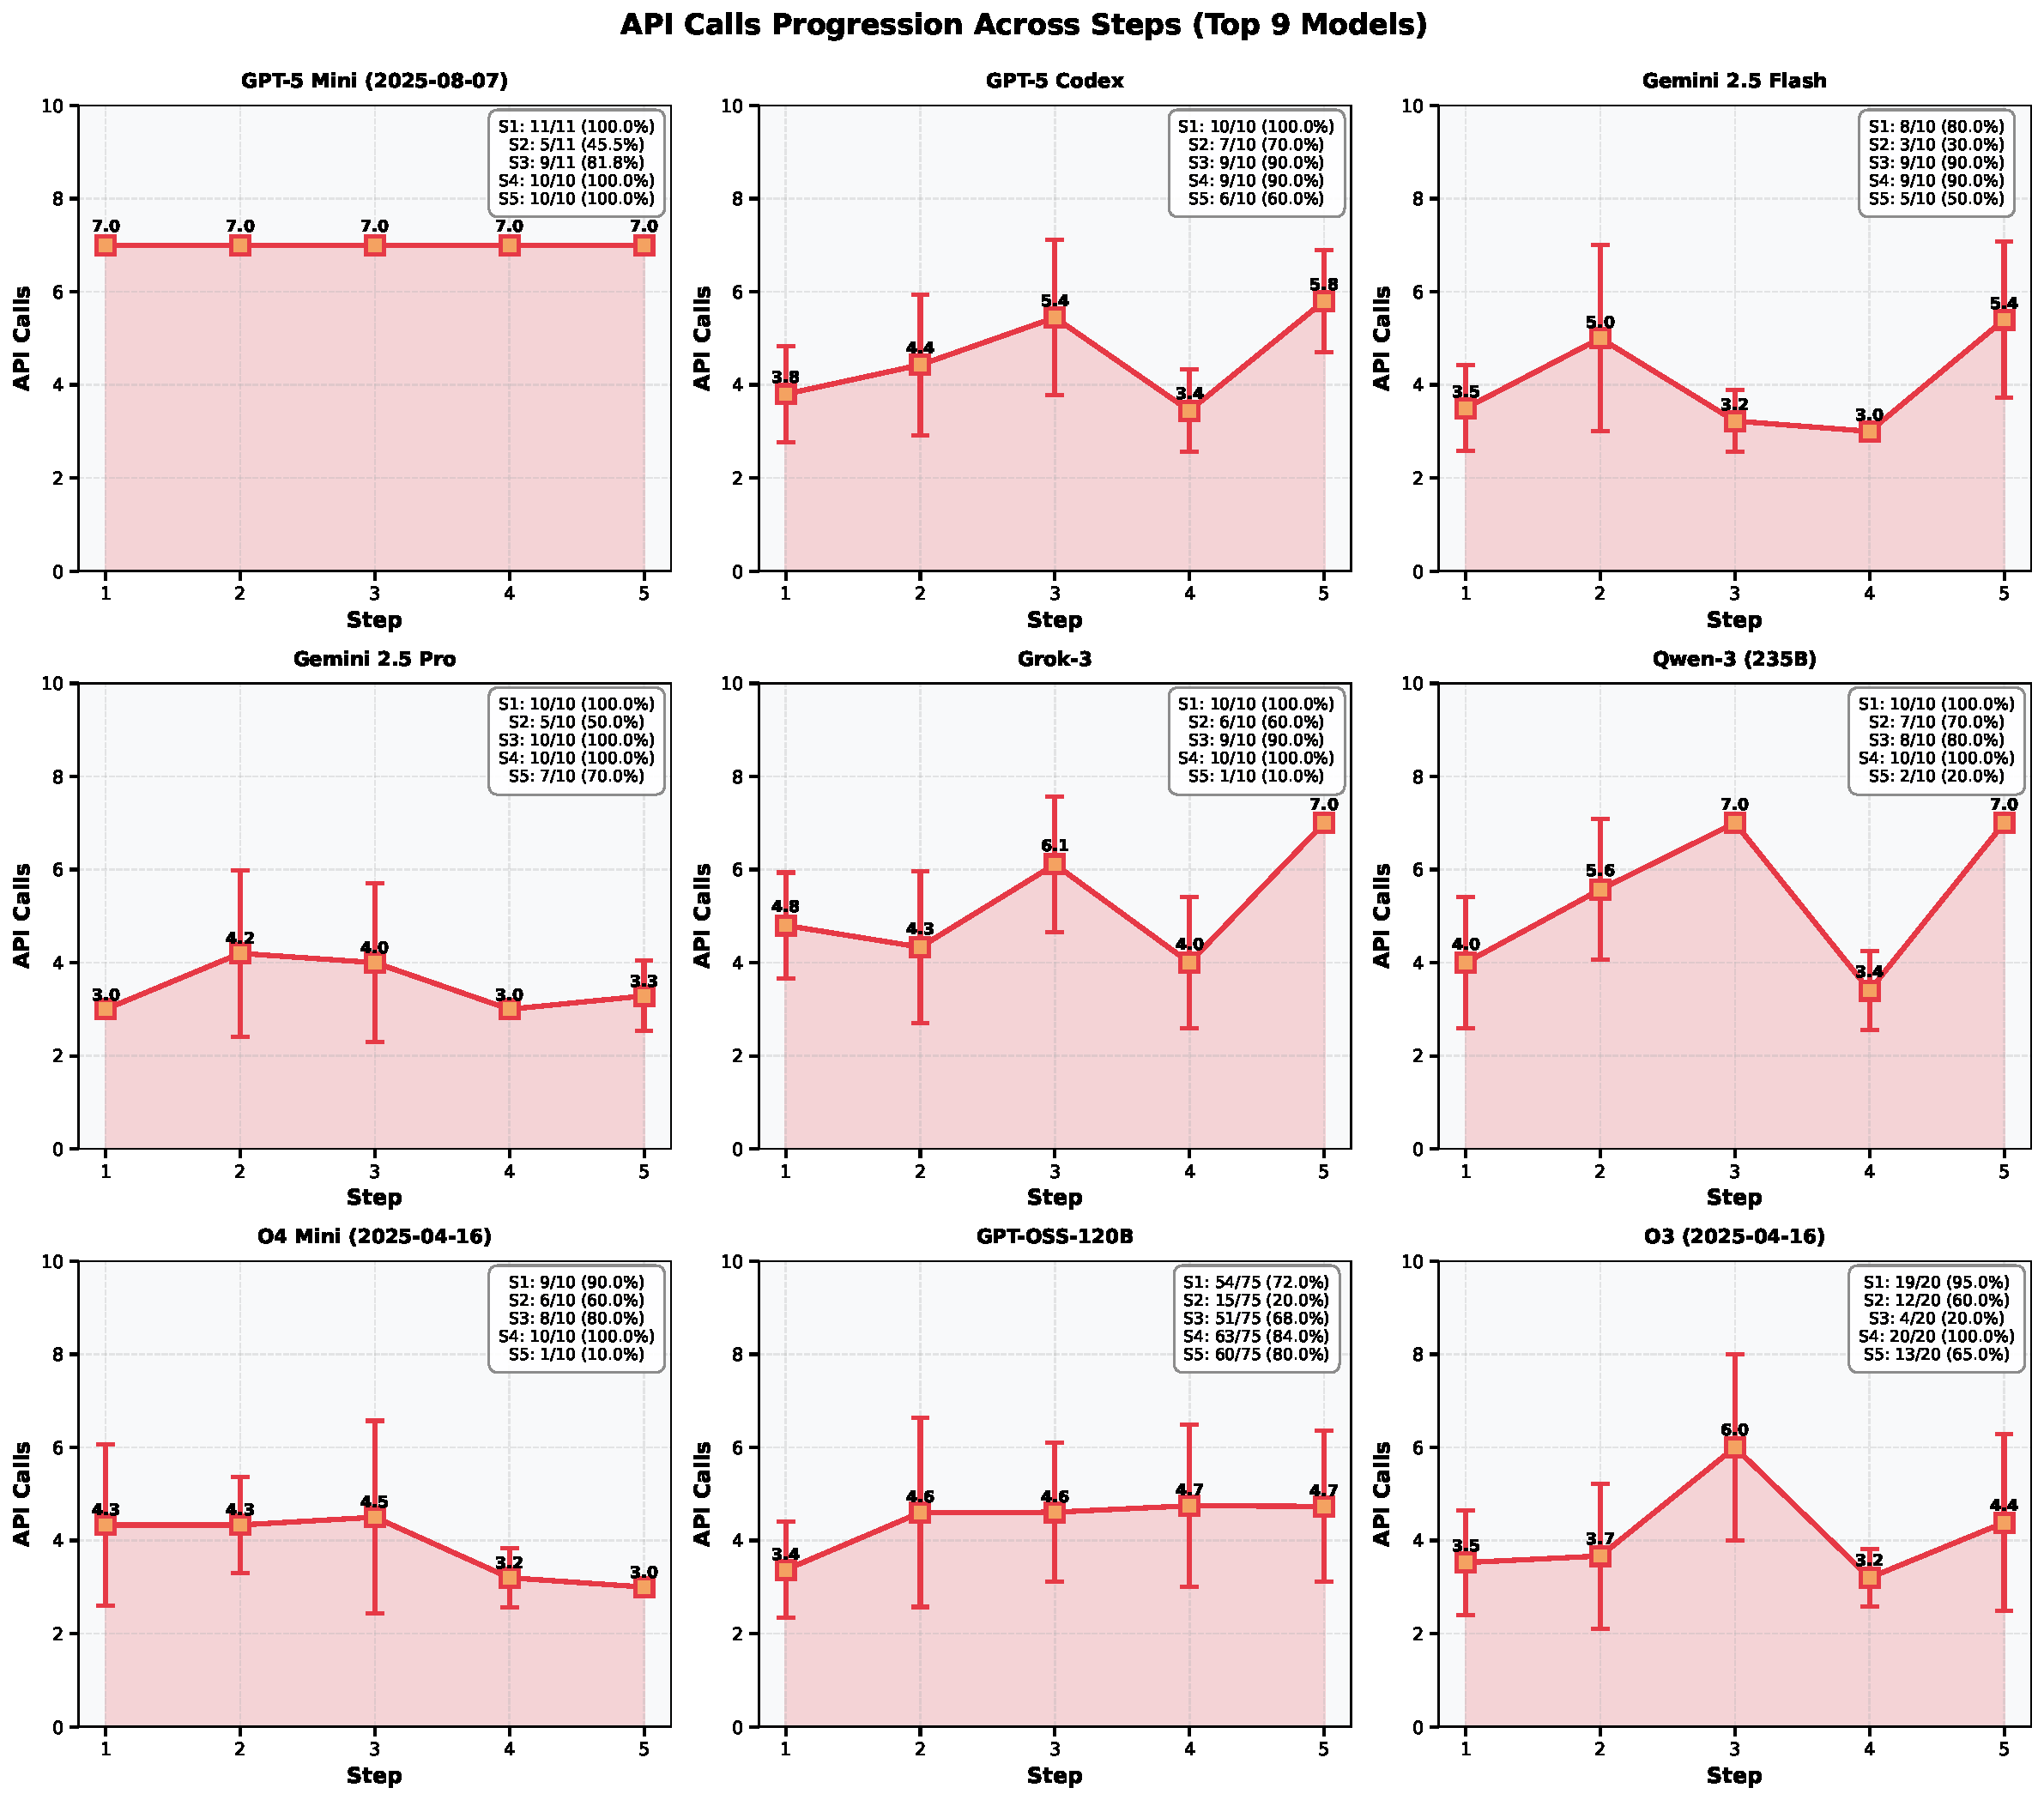
\includegraphics[width=0.95\textwidth]{3_api_calls_line_plot.pdf}
  \caption{
    \textbf{API-call progression across workflow steps.}
    Average API-call counts (with standard-deviation error bars) for the nine
    models that completed all workflow stages.
  }
  \label{fig:api_calls_progression}
\end{figure*}

\subsection{Various Measures}
\begin{figure*}[htbp]
  \centering
  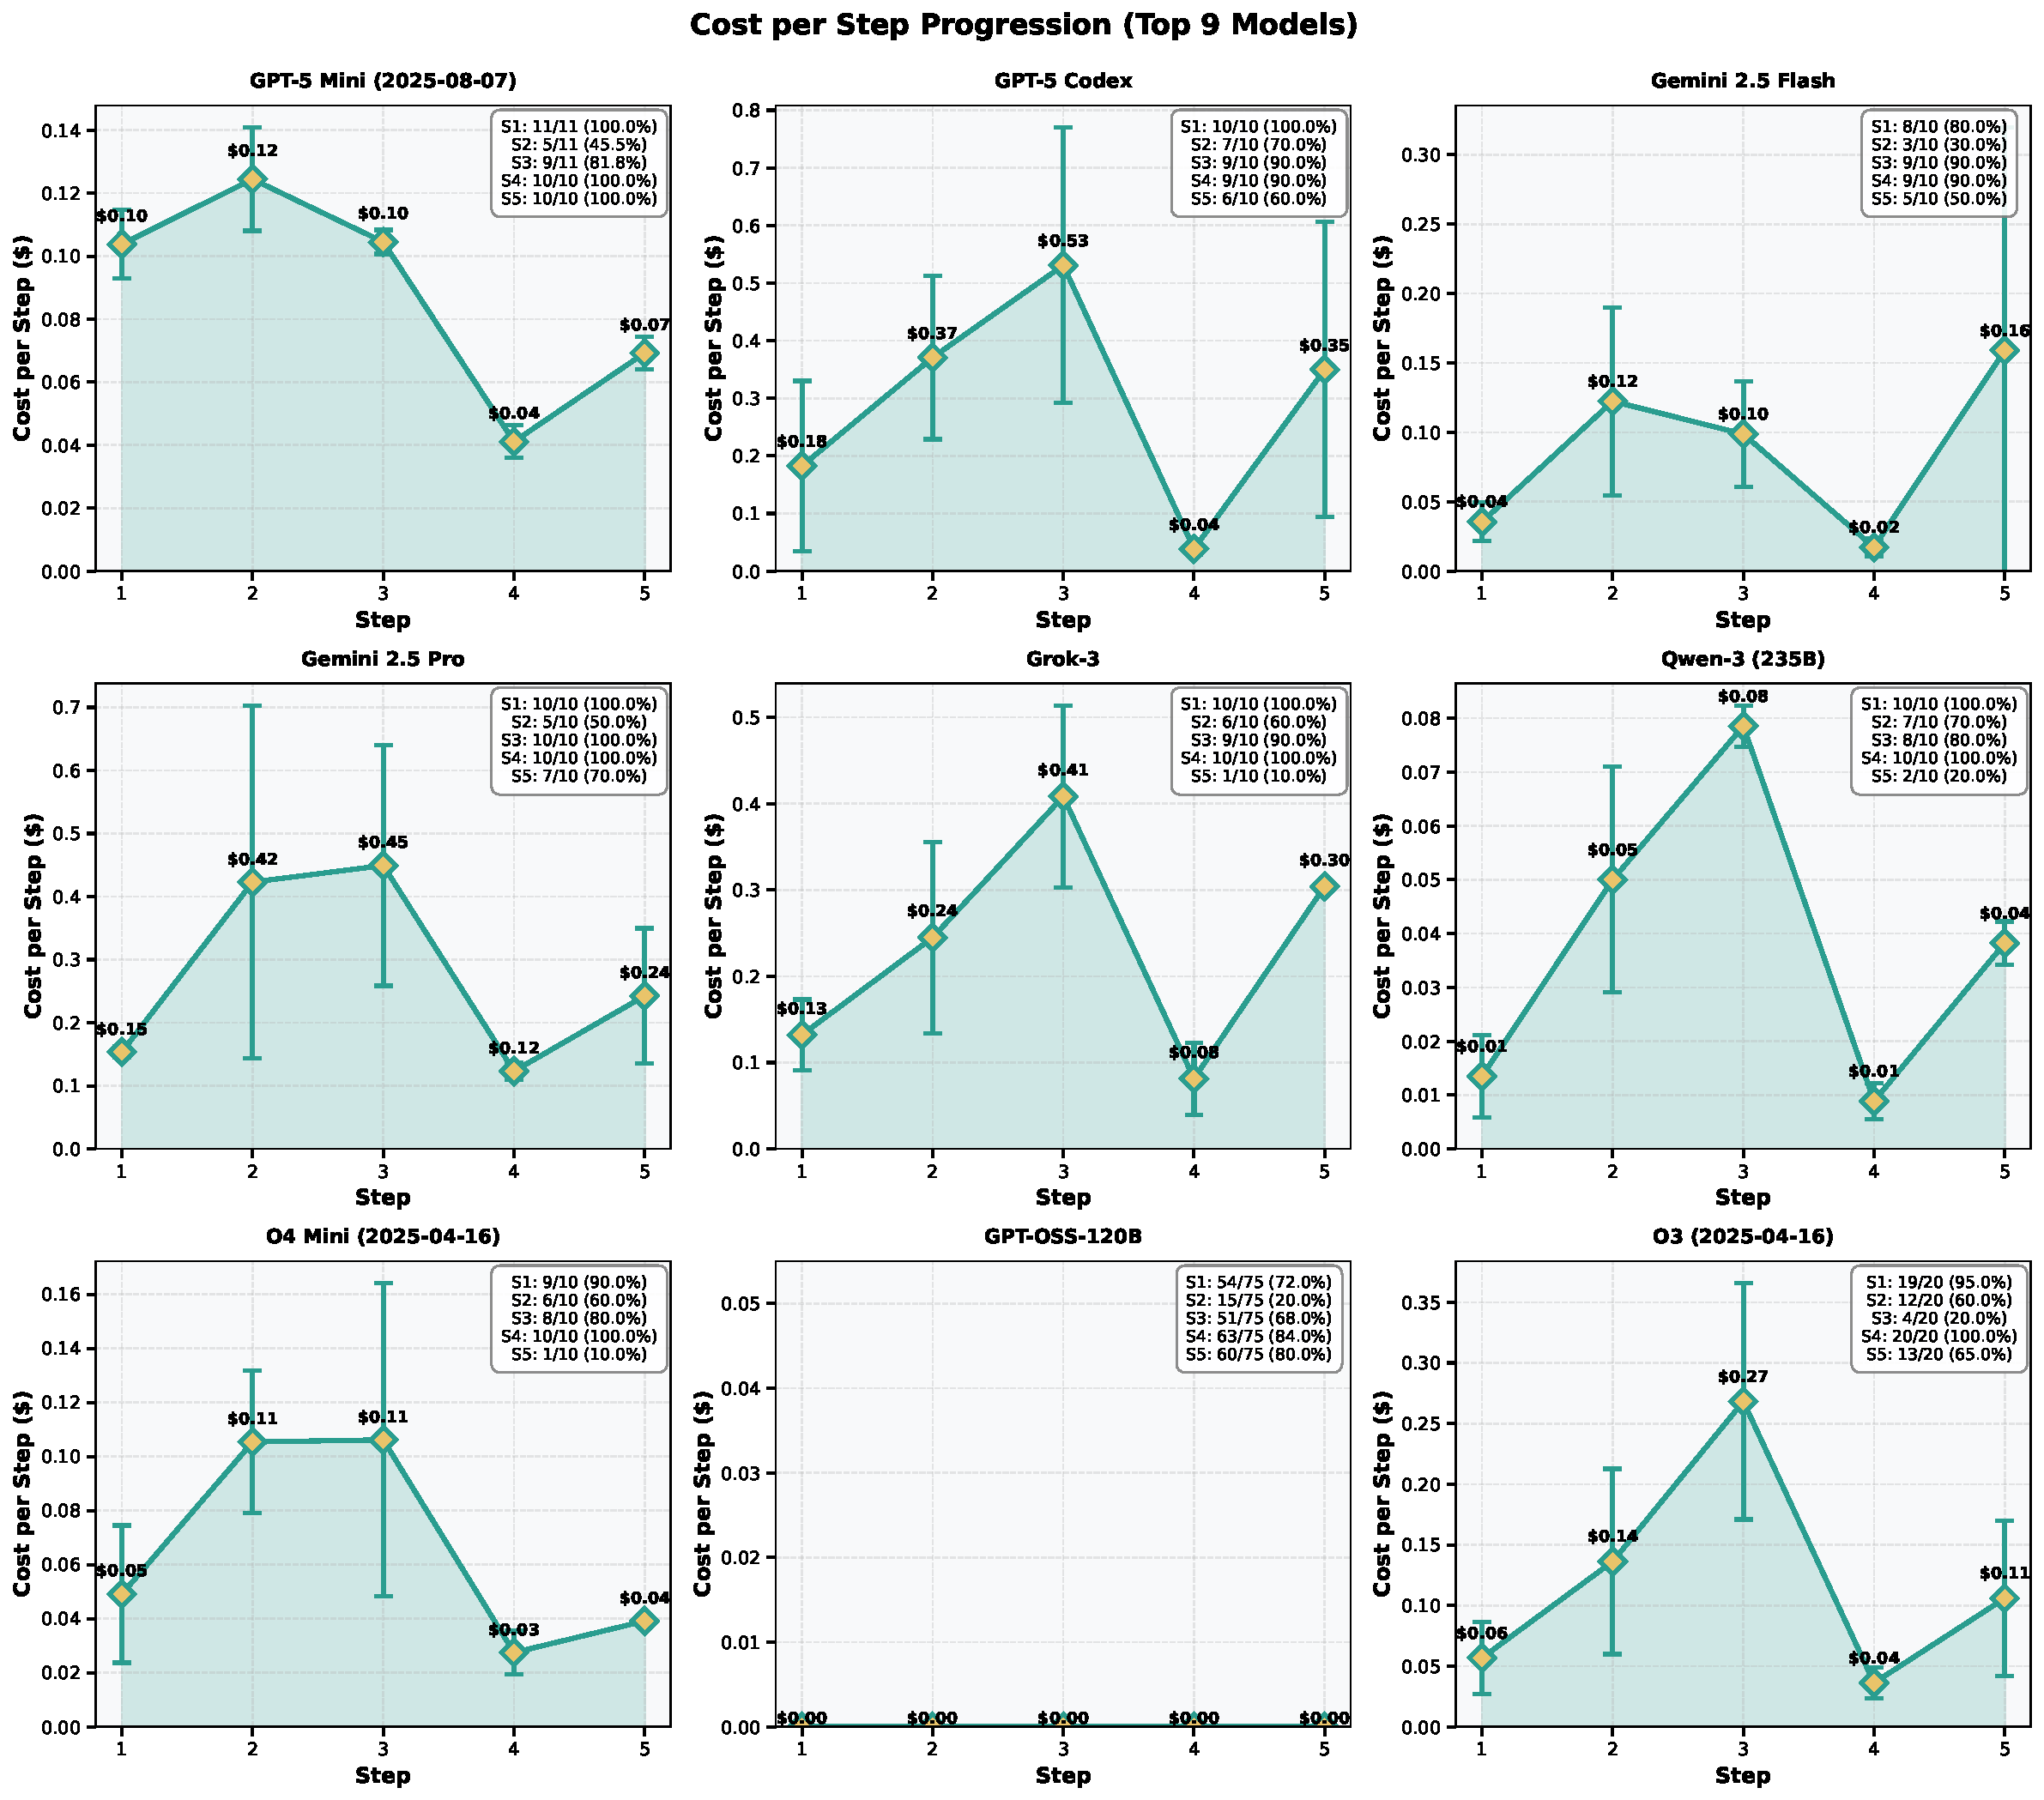
\includegraphics[width=0.95\textwidth]{4_cost_per_step.pdf}
  \caption{
    \textbf{Cost per analysis step across models.}
    The estimated dollar cost per step is computed from the observed token usage 
    and the publicly listed pricing for each model configuration, shown in Appedix~\ref{appendix:model_api_cost}. This metric 
    captures the effective economic cost of completing the workflow. 
    Higher-capacity models tend to combine lower agent work with higher dollar 
    cost, whereas smaller or open-weight models offer lower absolute cost but 
    substantially reduced reliability.
  }
  \label{fig:cost_per_step}
\end{figure*}
Figure~\ref{fig:agent_work}, Figure~\ref{fig:api_calls_progression}, and Figure~\ref{fig:cost_per_step} summarize results for a subset of the models tested. Although 20 models were evaluated in total (see Figure~\ref{fig:success_heatmap}), only nine achieved at least one successful completion in \emph{every} step of the workflow. We restrict the quantitative comparisons in these figures to this subset to ensure a fair and well-defined evaluation: metrics such as agent work, API-call behavior, and effective cost are meaningful only when a model is capable of completing the entire pipeline. Including models that never reached certain stages would bias these measurements and obscure true performance differences. The nine consistently successful models therefore constitute the evaluation set for the comparative analysis.
%Figure~\ref{fig:agent_work}, Figure~\ref{fig:api_calls_progression}, and Figure~\ref{fig:cost_per_step} include only the nine models that achieved at least one successful completion in every step of the workflow. These models form the evaluation set for comparing agent work, API-call behavior, and effective cost across the pipeline.

% \begin{figure}[htbp]
%   \centering
%   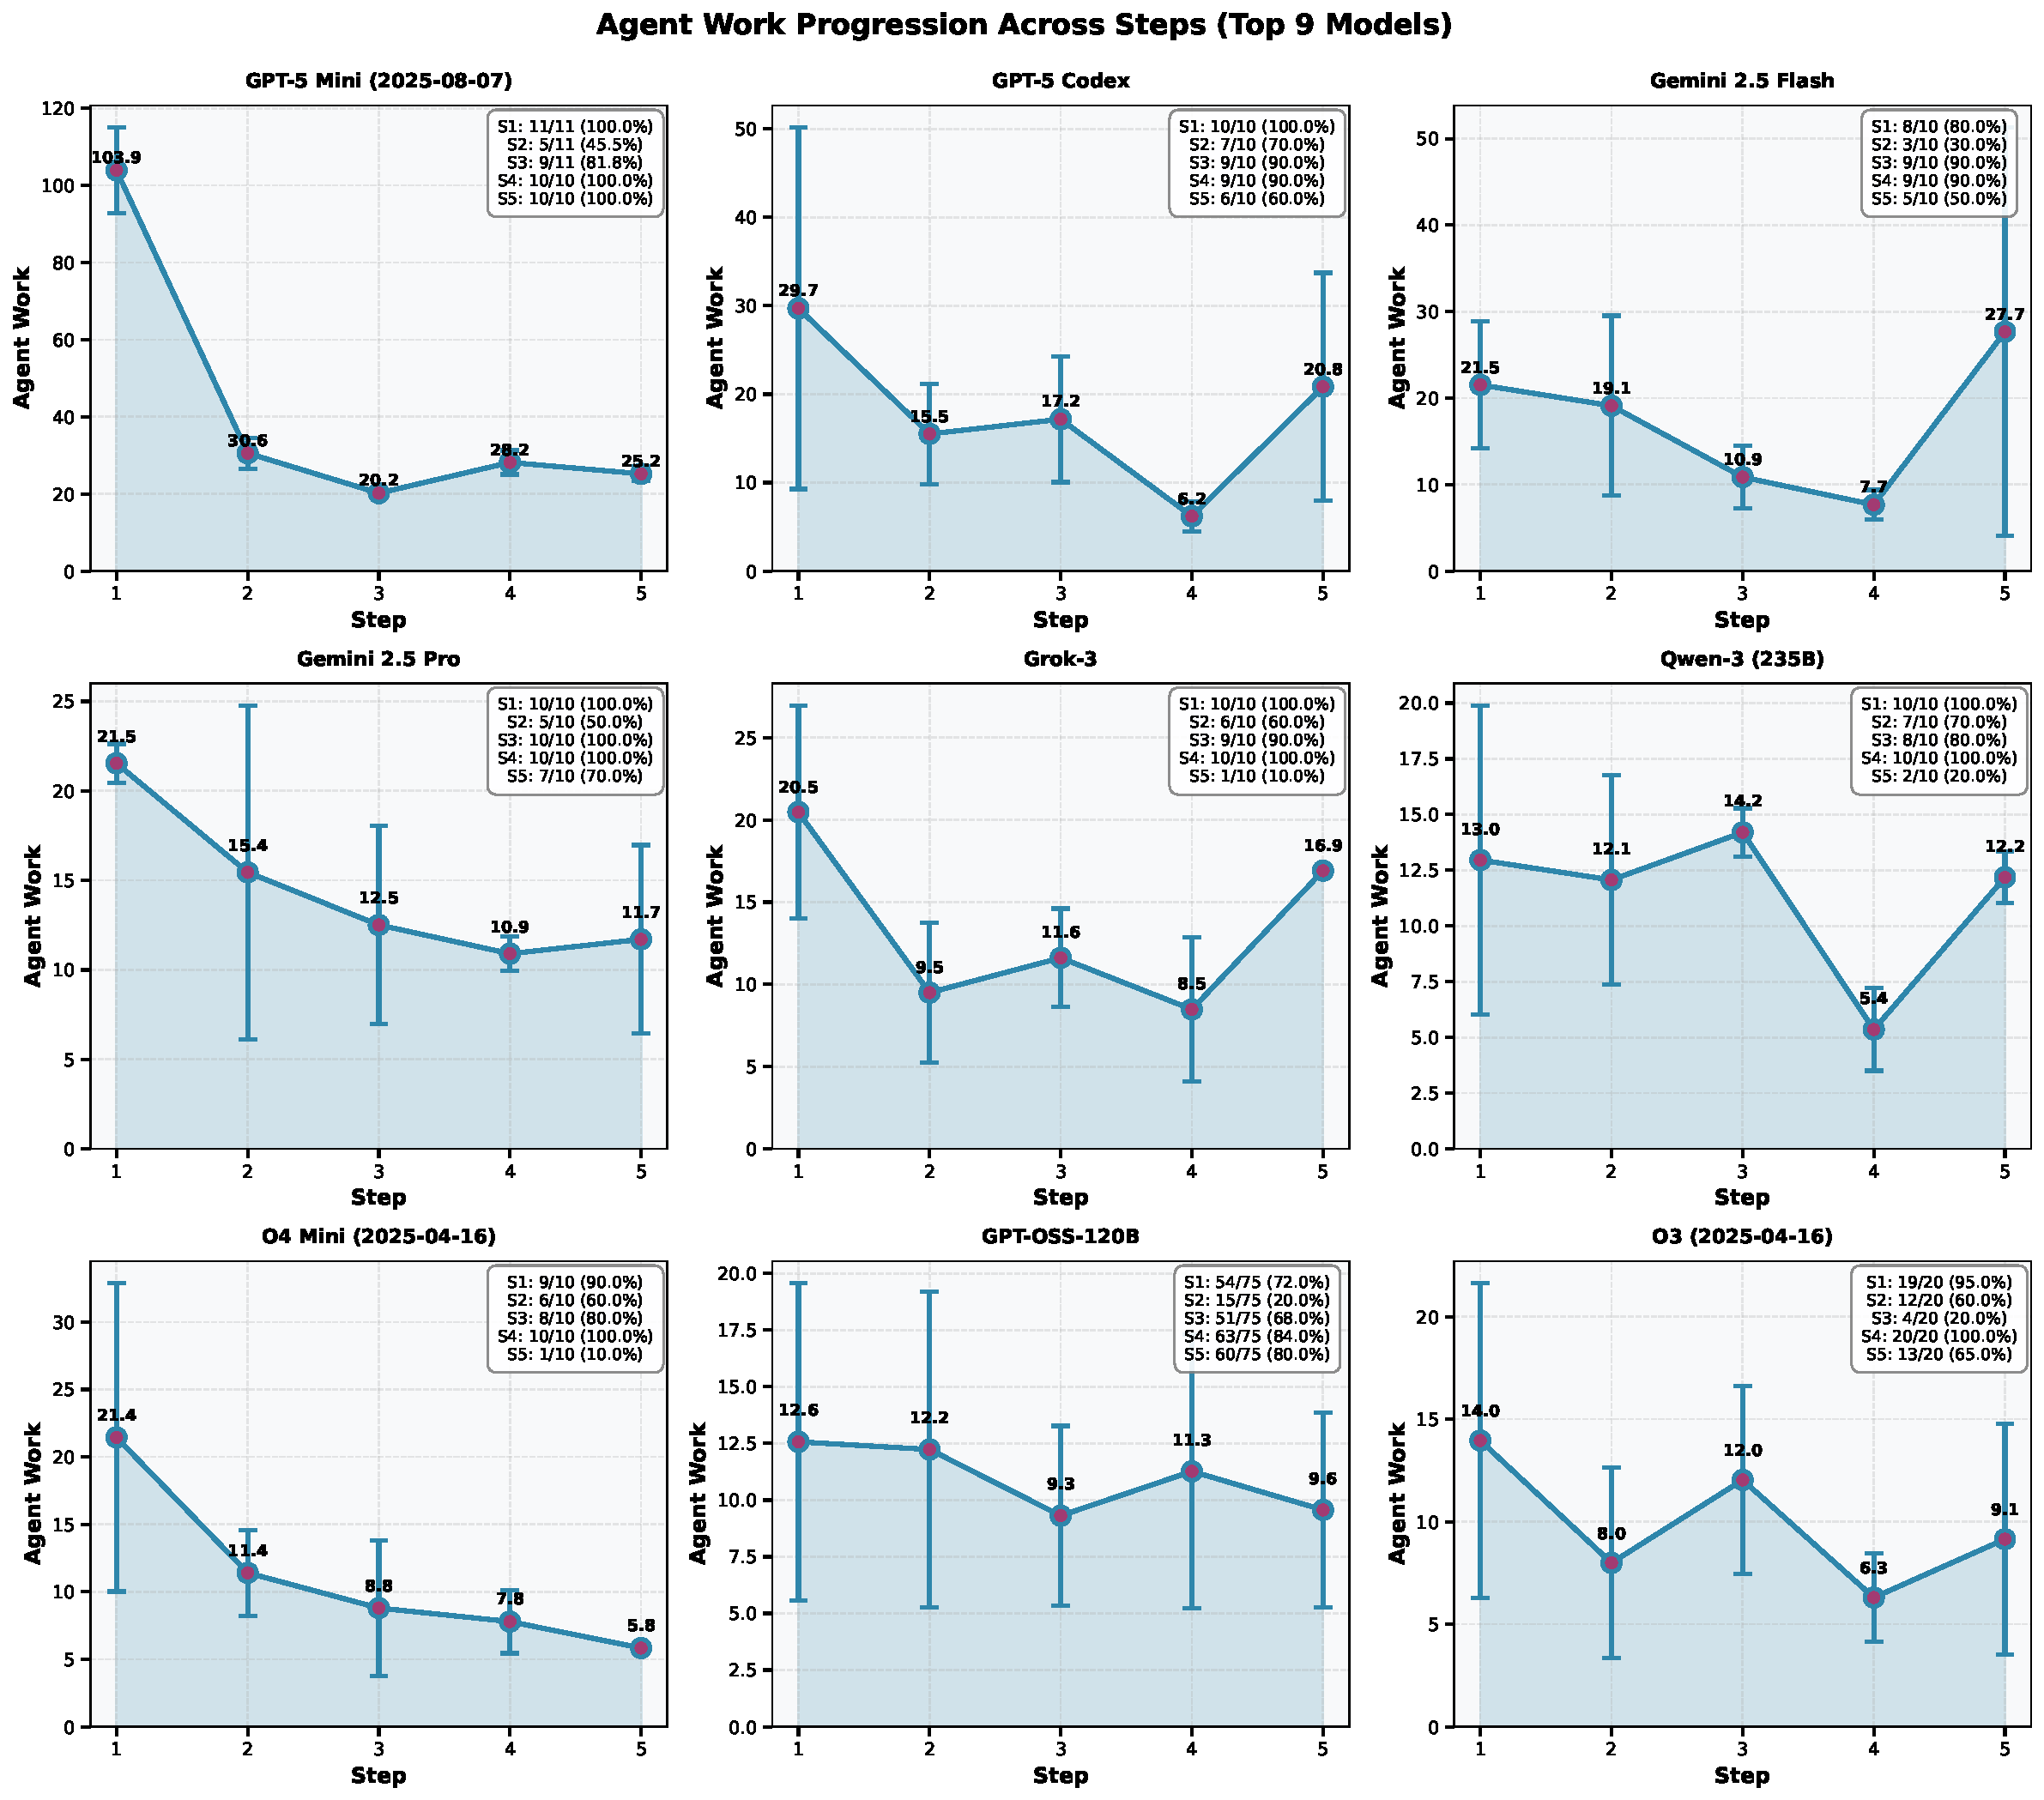
\includegraphics[width=0.9\columnwidth]{2_agent_work_line_plot.pdf}
%   \caption{
% \textbf{Agent work progression across workflow steps.}
% Average agent work (with standard-deviation error bars) shown for the nine
% models that successfully completed all stages of the workflow.
% }
%   \label{fig:agent_work}
% \end{figure}
%Figure~\ref{fig:agent_work} presents the agent work metric, defined as \textit{Agent Work} = (\textit{Total Tokens} -- \textit{User Tokens}) / \textit{User Tokens}, which quantifies how much autonomous reasoning and internal iteration the agent performs beyond the initial human prompt. As seen in the uploaded plots, agent work varies substantially across models and steps: some models rely on large bursts of internal prompting during early steps but stabilize later, while others show more uniform iteration patterns throughout the workflow. Notably, models with high completion rates in Figure~\ref{fig:success_heatmap} do not necessarily achieve low agent work, indicating that reliability can arise either through strong single-pass reasoning or through extensive internal repair.
Figure~\ref{fig:agent_work} shows the agent work metric across workflow stages for the nine models that successfully completed all steps of the pipeline. Agent work is defined as
\begin{equation*}
    \text{Agent Work}\equiv\frac{\text{Total Tokens}-\text{User Tokens}}{\text{User Tokens}},
\end{equation*}
and measures the amount of autonomous reasoning, internal iteration, and self-correction performed beyond the initial user instruction.

The standard-deviation error bars quantify the stability of the model’s reasoning behavior across repeated trials. Models with small uncertainties exhibit highly consistent internal prompting patterns, while larger error bars indicate more volatile behavior—often corresponding to inconsistent self-repair strategies or sensitivity to intermediate outputs. These collective trends provide insight not only into how much iteration a model performs, but how reliably it executes those iterative processes.

The agent-work curves reveal substantial variation across both models and workflow stages. Several models show large bursts of internal prompting during the data-preparation step - consistent with the high failure rate observed for this stage - before settling into more stable behavior in later steps where the task structure becomes clearer. Other models display nearly uniform agent-work profiles, suggesting steadier, more systematic reasoning strategies across the entire workflow. Importantly, high success rates in Figure~\ref{fig:success_heatmap} do not necessarily correspond to low agent work. Some models achieve reliability through strong single-pass reasoning with minimal iteration, while others succeed only after extensive internal repair. This diversity highlights that low agent work is not inherently synonymous with robustness; rather, it reflects a particular style of problem-solving that may or may not be advantageous depending on task structure.

% \begin{figure*}[htbp]
%   \centering
%   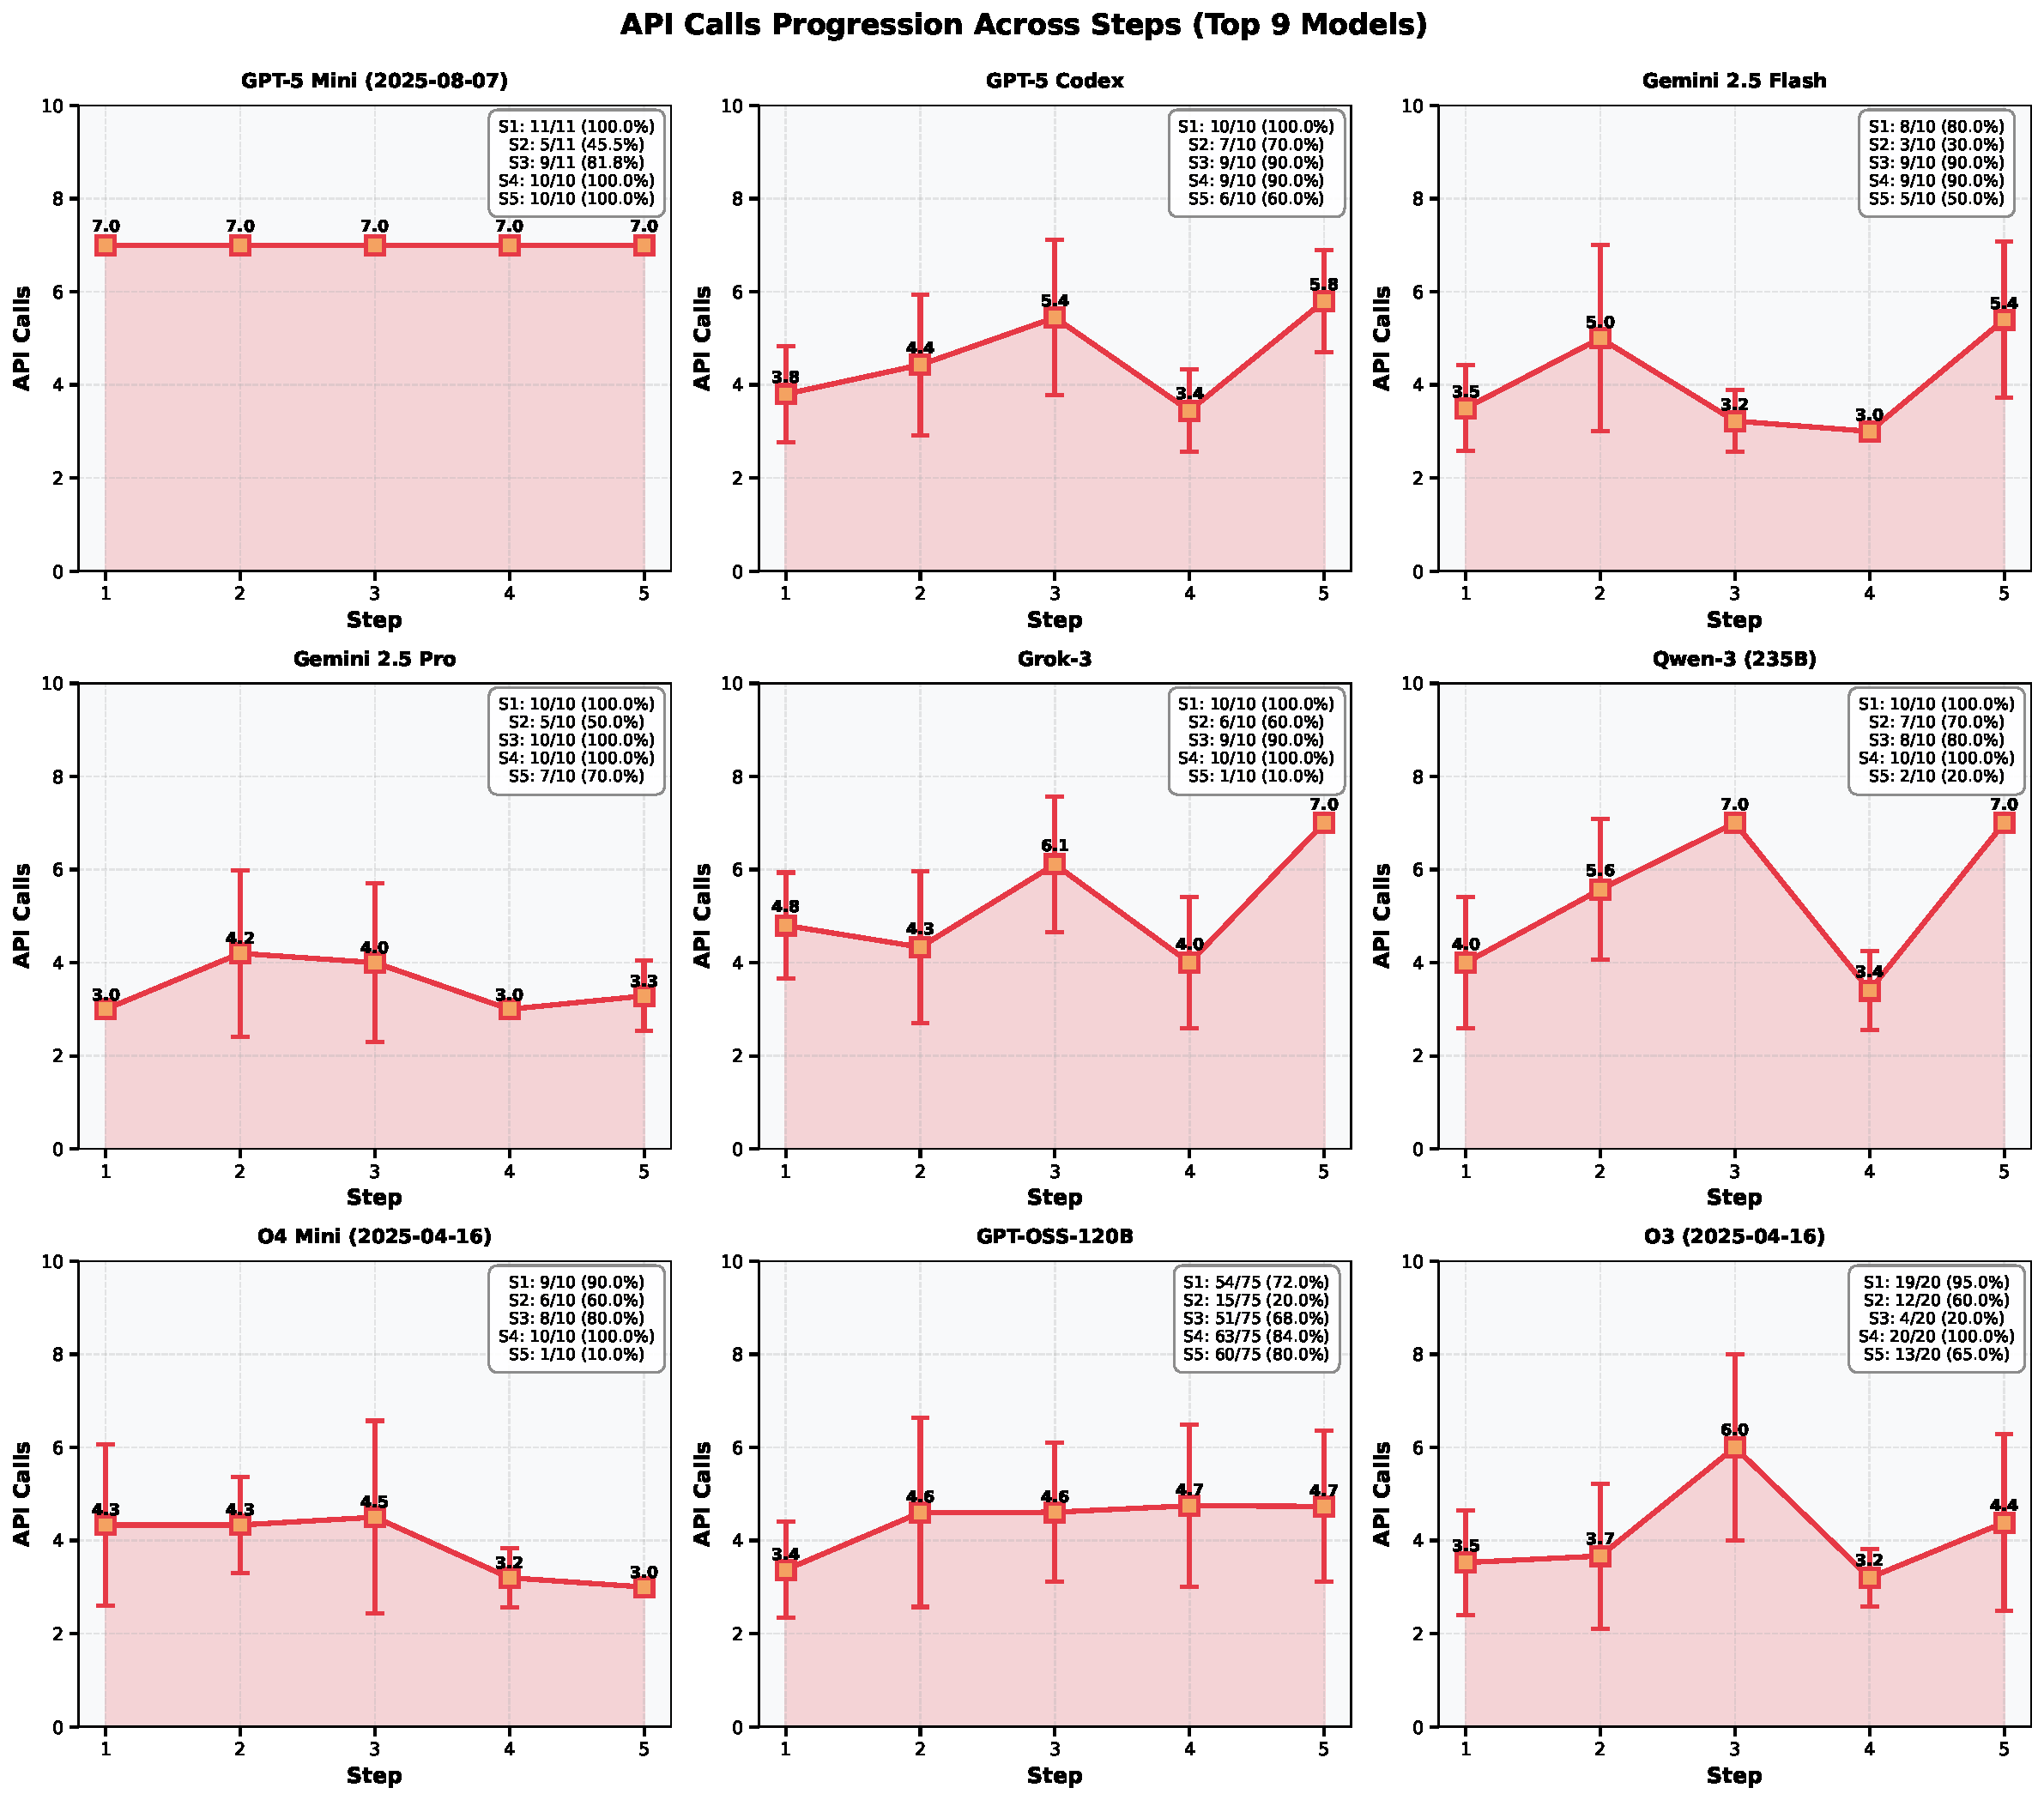
\includegraphics[width=0.95\columnwidth]{3_api_calls_line_plot.pdf}
%   \caption{
% \textbf{API-call progression across workflow steps.}
% Average API-call counts (with standard-deviation error bars) for the nine
% models that completed all workflow stages.
% }\label{fig:api_calls_progression}
% \end{figure*}

%Figure~\ref{fig:api_calls_progression} reports the number of API calls issued by the agent at each workflow step. In our setup, the agent is allowed up to three corrective attempts per step; this corresponds to a maximum of seven API calls in total: one initial call to the supervisor, followed by up to three supervisor–coder interaction cycles, each consisting of a pair of calls (one from the supervisor to the coder and one returning the coder’s output). These API calls represent discrete model-query events and therefore provide a complementary view of the agent’s iteration dynamics. Some models maintain relatively stable API-call counts across all steps, while others exhibit substantial fluctuations, revealing difficulties that are localized to specific analysis stages. Taken together with Figure~\ref{fig:agent_work}, these results demonstrate that high internal reasoning effort does not necessarily imply frequent external API interactions—and conversely, that models may iterate externally without engaging in extensive internal self-correction.
Figure~\ref{fig:api_calls_progression} reports the number of API calls issued by the agent at each workflow step for the nine models that successfully completed the entire pipeline. In our setup, an agent may attempt up to three corrective retries per step, corresponding to a maximum of seven API calls: one initial supervisor call followed by as many as three supervisor–coder interaction cycles. Whereas the agent-work metric captures internal reasoning effort, API-call counts measure how frequently the agent must rely on external interactions with the model to make progress.

The error bars quantify run-to-run variability and reveal differences in the stability of each model’s retry behavior. Some models maintain nearly constant API-call counts across all steps, indicating predictable correction strategies and consistent handling of intermediate failures. By contrast, several models exhibit higher API-call counts during the \textbf{categorization} stage, along with increased variability, suggesting that models find the optimization and decision-boundary logic in this stage particularly challenging. In comparison, data preparation generally requires fewer external interactions, reflecting its more structured and procedural character.

Overall, the API-call patterns highlight substantial diversity in how models manage uncertainty, recover from errors, and decide when external intervention is necessary. Some rely on frequent, lightweight retries, while others issue fewer but more targeted calls. These differences in external iteration behavior have direct implications for computational cost and operational efficiency, motivating the cost-per-analysis-step comparison presented next.

Figure~\ref{fig:cost_per_step} presents the estimated monetary cost per workflow step, computed by converting the observed token usage into dollars using publicly listed pricing for each model (Appendix \ref{appendix:model_api_cost}). Because each workflow stage involves different degrees of internal reasoning and external interaction, the resulting cost patterns provide insight into the computational demands of each step. Across nearly all models, the \textbf{preprocessing} stage is the most expensive. This reflects the substantial internal prompting, early error handling, and multi-step reasoning required for operations such as ROOT file inspection, ntuple construction, and initial event filtering. In contrast, the \textbf{S–B separation} step is consistently inexpensive, as it largely reduces to running a well-defined model-evaluation function with minimal iterative refinement. The \textbf{categorization} stage shows greater model-to-model variability: some models complete it with minimal additional iteration, while others incur noticeably higher cost due to repeated boundary adjustments and optimization retries.

The differences across models illustrate a clear capability–cost trade-off. Higher-capacity proprietary models often achieve lower agent work and more stable retry behavior, but these advantages come with higher per-token pricing, resulting in significantly elevated per-step cost. Smaller or open-weight models generally appear cheaper, but their reduced robustness can lead to inconsistent iteration patterns and occasional spikes in token usage. These trends emphasize that a model’s nominal price is only part of the story; the true operational cost depends on how efficiently the model navigates the reasoning and correction cycles required by each workflow stage.

A special case in Figure~\ref{fig:cost_per_step} is \texttt{gpt-oss-120b}, which appears with an effective cost close to zero. This stems from its execution on LBNL’s CBorg infrastructure~\citep{cborg}, where inference cost is extremely low (essentially zero). This highlights the appealing economic profile of open-weight models when deployed on institutional compute resources, though such low marginal cost does not necessarily imply reliability or performance comparable to commercial systems. Overall, the cost patterns show that the effective economic footprint of an agent depends jointly on model pricing and the internal and external iteration dynamics needed to successfully complete each stage of the scientific workflow.
%Figure~\ref{fig:cost_per_step} converts the observed token usage into an estimated per-step monetary cost using each model's public pricing. A clear trade-off is visible: models with low agent work and more stable API-call patterns generally incur higher per-step cost, while smaller or open-weight models remain inexpensive but display higher variability, lower reliability, or both. These results illustrate that cost efficiency depends not only on nominal model pricing, but also on the internal and external iteration dynamics required to complete the workflow successfully.

\section{Limitations}
This study shows that LLMs can support HEP data analysis workflows by interpreting natural language, generating executable code, and applying basic self-correction. While multi-step task planning is beyond the current scope, the \texttt{Snakemake} integration provides a natural path toward rule-based agent planning. Future work will pursue this direction and further strengthen the framework through improvements in prompting, agent design, domain adaptation, and retrieval-augmented generation.
%This study illustrates how LLMs can be applied to computational HEP tasks that require interpreting natural language, generating executable code, and performing basic self-correction. Although multi-step task planning is not addressed in the present work, the integration with Snakemake naturally enables future extensions toward rule-based agent planning. Upcoming efforts will focus on this direction, as well as on enhancing the framework through advances in prompt engineering, agent design, domain adaptation, and retrieval-augmented generation.
%This work demonstrates the use of LLMs for computational HEP tasks involving natural language interpretation, code generation, and self-correction. While multi-step task planning is not explored here, the integration with Snakemake provides a natural pathway for extending the framework to rule-based agent planning. Future studies will investigate this direction, along with improvements from advances in prompt design, agent configuration, domain adaptation, and retrieval-augmented generation.
%This work focuses on developing LLMs to perform computational HEP tasks by interpreting natural language input, generating code, and self-correcting errors. We do not study multi-step, multi-turn task planning, though the use of Snakemake as a workflow manager provides a natural output format for such agents. Future work will investigate task planning expressed as Snakemake rules.

% Agentic AI is rapidly evolving, with active research in prompt engineering, agent configuration, domain-specific fine-tuning, and retrieval-augmented generation (RAG). These methods could further improve the effectiveness and efficiency of the system described here, and we leave such refinements to future studies.


\section{Conclusion}
We demonstrated the feasibility of employing LLM agents to automate components of high-energy physics (HEP) data analysis within a reproducible workflow. The proposed hybrid framework combines LLM-based task execution with deterministic workflow management, enabling near end-to-end analyses with limited human oversight. While the \texttt{gemini-pro-2.5} model served as a statistically stable reference, the broader cross-model evaluation shows that several contemporary LLMs can perform complex HEP tasks with distinct levels of reliability and robustness. Beyond this proof of concept, the framework provides a foundation for systematically assessing and improving LLM-agent performance in domain-specific scientific workflows.
%We demonstrated the feasibility of using LLM agents to automate HEP data analysis within a reproducible workflow.
%The proposed hybrid system integrates LLM-driven task execution with deterministic workflow management, enabling end-to-end analysis with minimal human intervention.While the \texttt{gemini-pro-2.5} model provided statistically robust benchmarks, the extended cross-model study highlights that multiple contemporary LLMs can complete complex HEP tasks with varying degrees of reliability, efficiency, and cost. Beyond this proof of principle, the framework establishes a general testbed for quantitatively evaluating and improving LLM-agent performance in domain-specific scientific workflows.
%We demonstrated the feasibility of using an LLM agent to automate HEP data analysis. The system is built on a hybrid architecture where LLM agents complete specific tasks at the request of human users, while a workflow manager orchestrates the sequential analysis steps. We evaluated the performance of the \texttt{gemini-2.5-pro} model with the agentic analysis workflow.  Beyond serving as a proof-of-principle study, this framework can be further developed into a testbed for assessing the ability of different LLMs to automate HEP-specific analysis tasks.

\section*{Acknowledgement}
This work was supported by the U.S. Department of Energy (DOE), Office of Science (SC), under Award No. DE-SC0023718.  Gendreau-Distler’s contribution was partially supported by the U.S. National Science Foundation under Award No. 2046280. Wang's contribution was partially supported by the DOE SC under the Contract No. DE-AC02-05CH11231. This research used the CBorg AI platform and resources provided by the IT Division at the Lawrence Berkeley National Laboratory (Supported by the Director, Office of Science, Office of Basic Energy Sciences, of the U.S.\ Department of Energy under Contract No.\ DE-AC02-05CH11231). The authors also thank Andrew Schmeder of LBNL’s IT Division for assistance with CBorg. This work additionally used resources of the National Energy Research Scientific Computing Center (NERSC), a DOE Office of Science User Facility operated under Contract No.\ DE-AC02-05CH11231. %This work also used resources of the National Energy Research Scientific Computing Center (NERSC), a DOE Office of Science User Facility, operated under Contract No. DE-AC02-05CH11231.

\newpage
\bibliographystyle{unsrtnat}
\bibliography{ref.bib}

\newpage
\appendix

\section{Technical Appendices and Supplementary Material}\label{appendix:physics_details}


% \subsection{Model summaries}

% \begin{description}

% \item[\texttt{aws\_llama-4-maverick}] Meta \textbf{Llama 4} (Maverick 17B) served via AWS Bedrock; family: \emph{Meta Llama}; \emph{open-weight}; not a dedicated “reasoning” model (general multimodal foundation model with strong reasoning ability).

% \item[\texttt{aws\_llama-4-scout}] Meta \textbf{Llama 4} (Scout 17B) on AWS Bedrock; family: \emph{Meta Llama}; \emph{open-weight}; not a dedicated “reasoning” model (general multimodal model with long-context capabilities).

% \item[\texttt{claude-3-5-haiku-20241022}] Anthropic \textbf{Claude 3.5 Haiku}; family: \emph{Claude}; \emph{closed-weight}; not a specialized reasoning model (optimized for speed with capable reasoning).

% \item[\texttt{claude-sonnet-4-20250514}] Anthropic \textbf{Claude Sonnet 4}; family: \emph{Claude}; \emph{closed-weight}; \emph{hybrid/advanced reasoning} model.

% \item[\texttt{llama}] Meta \textbf{Llama} family (generic entry); family: \emph{Meta Llama}; typically \emph{open-weight}; not a dedicated reasoning model (general-purpose LLM).

% \item[\texttt{openai\_gpt-5}] OpenAI \textbf{GPT-5} system (includes GPT-5 \emph{Thinking} and GPT-5 \emph{Main}); family: \emph{OpenAI}; \emph{closed-weight}; \emph{reasoning} when using the Thinking variants.

% \item[\texttt{o4-mini}] OpenAI \textbf{o4-mini}; family: \emph{OpenAI o-series}; \emph{closed-weight}; \emph{reasoning} model optimized for speed/cost.

% \item[\texttt{gemini-2.5-pro}] Google DeepMind \textbf{Gemini 2.5 Pro}; family: \emph{Gemini}; \emph{closed-weight}; \emph{hybrid reasoning} model.

% \item[\texttt{gemini-2.5-flash}] Google DeepMind \textbf{Gemini 2.5 Flash}; family: \emph{Gemini}; \emph{closed-weight}; \emph{hybrid reasoning} model tuned for low-latency use.

% \item[\texttt{gemini-2.0-flash-lite}] Google DeepMind \textbf{Gemini 2.0 Flash-Lite}; family: \emph{Gemini}; \emph{closed-weight}; lightweight non-flagship model (not branded as a dedicated reasoning model, but supports basic reasoning).

% \item[\texttt{gcp\_qwen-3-coder}] Alibaba \textbf{Qwen3 Coder}; family: \emph{Qwen}; \emph{open-weight}; code-specialized model with optional \emph{“Thinking”} (reasoning) mode.

% \item[\texttt{gcp\_qwen-3}] Alibaba \textbf{Qwen3}; family: \emph{Qwen}; \emph{open-weight}; general model with \emph{hybrid “Thinking/Non-Thinking”} reasoning modes.

% \item[\texttt{gpt-oss-120b}] OpenAI \textbf{gpt-oss-120b}; family: \emph{OpenAI gpt-oss}; \emph{open-weight}; Mixture-of-Experts \emph{reasoning} model intended for high-reasoning, production use.

% \item[\texttt{openai\_o3}] OpenAI \textbf{o3}; family: \emph{OpenAI o-series}; \emph{closed-weight}; frontier \emph{reasoning} model.

% \item[\texttt{gpt-oss-20b}] OpenAI \textbf{gpt-oss-20b}; family: \emph{OpenAI gpt-oss}; \emph{open-weight}; smaller MoE \emph{reasoning} model suitable for local/edge deployment.

% \item[\texttt{openai\_gpt-5-mini}] OpenAI \textbf{GPT-5 mini}; family: \emph{OpenAI}; \emph{closed-weight}; “mini” variants exist for both \emph{Thinking} (reasoning) and \emph{Main} (non-reasoning) configurations.

% \item[\texttt{claude-opus-4-1}] Anthropic \textbf{Claude Opus 4.1}; family: \emph{Claude}; \emph{closed-weight}; flagship \emph{reasoning} model for complex, agentic tasks.

% \item[\texttt{openai\_o3-mini-high}] OpenAI \textbf{o3-mini-high}; family: \emph{OpenAI o-series}; \emph{closed-weight}; \emph{reasoning} variant running with high reasoning effort.

% \item[\texttt{xai\_grok-3}] xAI \textbf{Grok 3}; family: \emph{xAI Grok}; \emph{closed-weight}; \emph{reasoning} model (beta) emphasizing test-time thinking.

% \item[\texttt{xai\_grok-3-mini}] xAI \textbf{Grok 3 mini}; family: \emph{xAI Grok}; \emph{closed-weight}; lightweight \emph{reasoning} model optimized for cost/latency.

% \end{description}


\subsection{Features used for TabPFN classifier}
The language model is asked to save an extensive list of particle observables that would be useful for a more sophisticated physics analysis: the transverse momentum ($p_T$), pseudorapidity ($\eta$), and azimuthal angle ($\phi$) of the two leading photons, of the two leading leptons, and of the six leading jets; the transverse momentum and azimuthal angle of the missing transverse energy (MET); the Monte Carlo weight; the tight photon ID flags; the cross section; and the sum of Monte Carlo weights. However, in the interest of efficiency we use only the photon observables for the TabPFN classifier. The $p_T$ of photons are normalized by the invariant mass to prevent the classifier from learning to separate the signal and background events by the invariant mass. In addition, because only differences in azimuthal angle are physically meaningful, we replace the two diphoton $\phi$ coordinates with their difference $\phi_1 - \phi_2$.


\subsection{Event selection, training sample definition, and background estimation}

\paragraph{Preselection}  
To roughly follow the expected topology of a Higgs boson decaying into two photons, photon candidates are taken from well-calibrated regions of the detector ($|\eta| < 2.37$), while the transition zone between the barrel and endcap ($1.37 < |\eta| < 1.52$), where measurements are less reliable, is excluded. Each photon is required to have transverse energy above 25 GeV, ensuring that selected photons are energetic enough to be measured with good resolution and to suppress backgrounds from softer processes. Events are kept if they contain two photons that meet identification and isolation criteria, which help distinguish genuine photons from misidentified particles or nearby activity. To reflect the expected kinematics of Higgs decays, the leading photon must contribute more than 35\% of the diphoton system’s momentum ($p_T/m_{\gamma\gamma} > 0.35$), and the sub-leading photon more than 25\%. Finally, events are restricted to a diphoton invariant mass window of $105 < m_{\gamma\gamma} < 160$ GeV, a range chosen to capture the Higgs boson signal region while suppressing background contributions at much lower or higher masses.



\paragraph{Signal and background classifier training sample}  
Following the strategy of Ref.~\cite{ATLAS:2018mme}, events in which at least one photon does not meet the tight identification requirement are used to model the background in the signal region. These so-called NTI events are taken from the diphoton invariant mass sidebands, 105–120 GeV and 130-160 GeV, ranges chosen to minimize potential Higgs boson contributions. Because NTI events exhibit kinematic properties similar to those of tightly identified and isolated photons, they serve as a reliable proxy for background processes. For the signal sample, we use simulated Higgs boson events in which both photons satisfy the tight identification and isolation requirements. To ensure that the training is not biased toward either sample, signal and background events are rescaled to have equal weights.


\paragraph{Background estimate for sensitivity evaluation}  

To estimate the number of background events in the signal region (where both photons satisfy the tight isolation requirement), we rely on NTI events as a control sample. The signal is expected to appear as a narrow peak in the diphoton invariant mass distribution, so the significance is evaluated within a small mass window around the Higgs boson, $125 \pm 2$ GeV. The expected background in this window is inferred from the NTI sidebands using
\[
\text{Expected background} = SF1 \times SF2 \times NTI_{\text{yield}} .
\]  

In this expression, $NTI_{\text{yield}}$ denotes the number of NTI data events observed in the sideband regions. The scale factor $SF1$ accounts for the difference in yields between tight-isolated (TI) and NTI photons in the sidebands, while $SF2$ adjusts for the relative abundance of NTI events in the signal window compared with the sidebands. In this way, the measured background in the sidebands is extrapolated into the Higgs signal region. 



\subsection{Procedure of event categorization}
The goal of the event categorization is to select boundaries among $1000$ evenly spaced values of the signal-background separation score in a way that maximizes the statistical significance of the Higgs-to-diphoton signal process. We adopt a number counting significance formula given by
\[{\textstyle Z_i = \sqrt{2\left[(s_i + b_i)\ln{\left(1+\frac{s_i}{b_i}\right)}-s_i\right]}, \quad Z_{\text{tot}} = \sqrt{\sum_i Z_i^2}}\]

where summation runs over all categories and \(s_i/b_i\) denote numbers of signal/background events in \(i^{\text{th}}\) category. To maximize this significance, the first step is to scan over all possible locations for the boundary, compute the significance with each candidate boundary, and ultimately keep the boundary that yields the highest statistical significance. This procedure is then repeated until the most recently added boundary improves the overall significance by less than $5\%$.

\begin{figure}[h]
\centering
\begin{minipage}{0.48\textwidth}
    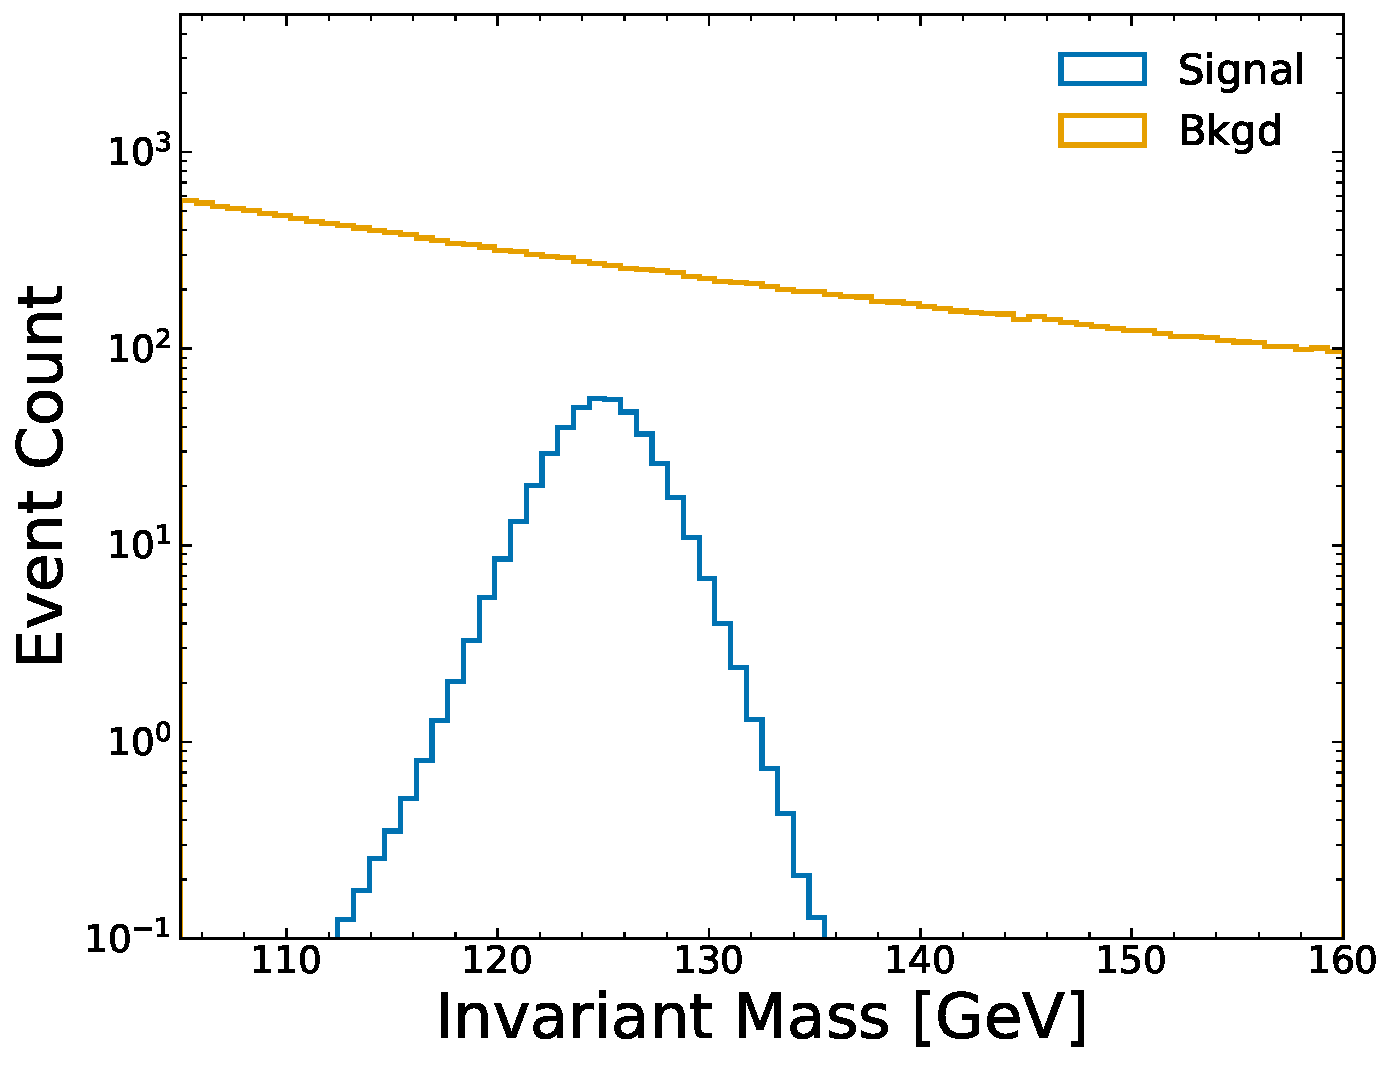
\includegraphics[height=0.8\textwidth]{myy.pdf}
\end{minipage}
\hfill
\begin{minipage}{0.48\textwidth}
    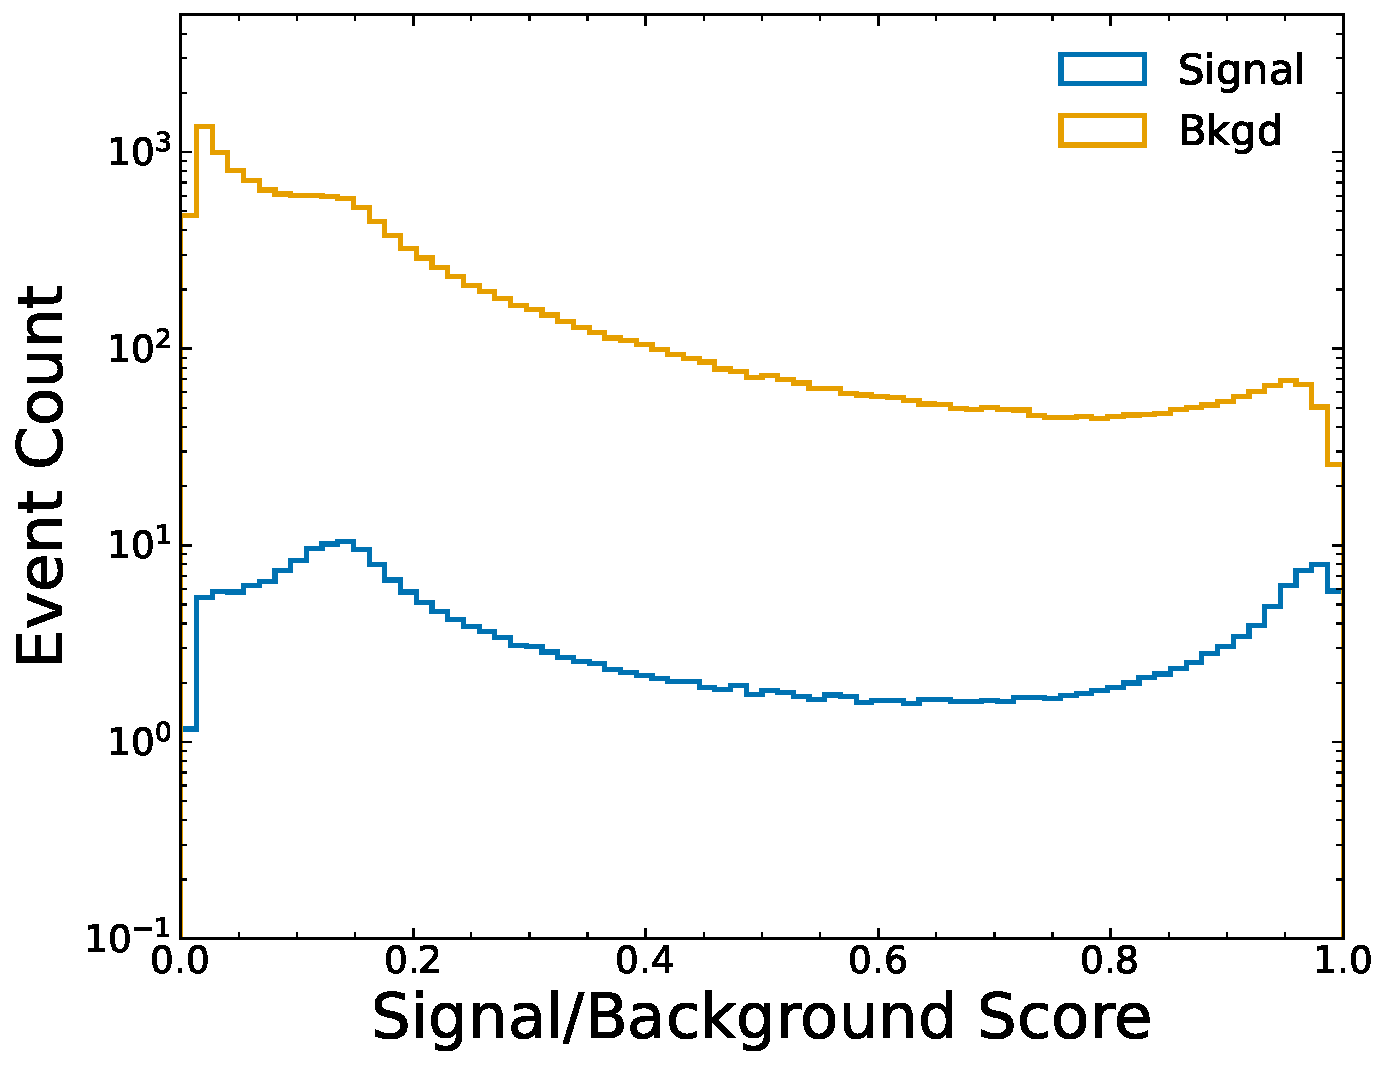
\includegraphics[height=0.8\textwidth]{scores.pdf}
\end{minipage}
\caption{Left: Invariant mass distribution of signal and background processes after standard analysis selections are applied. Right: Signal-background separation scores generated by TabPFN. Note that the normalization is different in the left and right plots because we apply cuts on the invariant mass before computing the signal-background separation scores.}
\label{fig:myy_scores}
\end{figure}

\section{Log Files and Error Analysis}\label{appendix:log_files_and_error_analysis}

\subsection{Comprehensive Log Example}

\lstinputlisting{comprehensive_log.txt}

\subsection{Validation Log Example}

\lstinputlisting{validation_log.txt}

\subsection{LLM-Error Analysis Example}
From the comprehensive log, we observe that the Supervisor/Coder was tasked with determining categorization boundaries to split events based on a classifier score. However, validation revealed that the boundaries selected did not exactly match those specified in the provided solution, leading to a failed trial. According to the LLM-based error analysis, this was classified as a \texttt{semantic error}, attributed to miscommunication between the User, Supervisor, and Coder. Specifically, the Supervisor misinterpreted the user's intent, and the Coder implemented instructions accordingly. 

A crucial difference emerged between the code generated by the Supervisor/Coder and the reference solution, namely, the solution initialized the \texttt{significances} array with the significance of the null selection (category boundaries at 0 and 1). In contrast, the Supervisor/Coder's approach did not include this initial step. This discrepancy led the LLM agent to add an extra boundary not present in the solution, ultimately producing five categorization boundaries instead of the four expected. As a result, the trial was marked as unsuccessful due to a semantic error.

\section{Model API Cost}\label{appendix:model_api_cost}
\begin{table}[htbp]
\centering
\begin{tabular}{|l|c|c|}
\hline
\textbf{Model} &
\shortstack{ \\ \textbf{Input Cost} \\ (\$/1M tokens)} &
\shortstack{\\ \textbf{Output Cost} \\ (\$/1M tokens)} \\
\hline
Claude 3.5 Haiku (2024-10-22)      & 0.80   & 15.00 \\
Claude Haiku 4.5 (2025-10-01)      & 1.00   & 5.00  \\
Claude Opus 4.1 (2025-08-05)       & 15.00  & 75.00 \\
Claude Sonnet 4.5 (2025-09-29)     & 3.00   & 15.00 \\
DeepSeek-R1                        & 0.28   & 0.42  \\
GPT-5 (2025-08-07)                 & 1.25   & 10.00 \\
GPT-5 Codex                        & 1.25   & 10.00 \\
GPT-5 Mini (2025-08-07)            & 0.25   & 2.00  \\
GPT-OSS-120B                       & 0.00   & 0.00    \\
Gemini 2.0 Flash Lite              & 0.10   & 0.40  \\
Gemini 2.5 Flash                   & 0.30   & 2.50  \\
Gemini 2.5 Pro                     & 1.25   & 10.00 \\
Grok Code Fast 1                   & 0.20   & 1.50  \\
Grok Mini                          & 0.30   & 0.50  \\
Grok-3                             & 3.00   & 15.00 \\
Llama-4 Maverick (17B)             & 0.50   & 2.00    \\
Llama-4 Scout (17B)                & 0.30   & 1.00    \\
O3 (2025-04-16)                    & 2.00   & 8.00  \\
O3 Mini (2025-01-31)               & 1.10   & 4.40  \\
O4 Mini (2025-04-16)               & 1.10   & 4.00  \\
Qwen-3 (235B)                      & 0.50   & 2.00    \\
\hline
\end{tabular}
\caption{Input and output costs for each model (in US dollars per 1M tokens). All cost values reflect the most recent updates as of October 2025.}\label{tab:model_api_cost}
\end{table}

%%%%%%%%%%%%%%%%%%%%%%%%%%%%%%%%%%%%%%%%%%%%%%%%%%%%%%%%%%%%

% \newpage
% \section*{NeurIPS Paper Checklist}

% \begin{enumerate}

% \item {\bf Claims}
%     \item[] Question: Do the main claims made in the abstract and introduction accurately reflect the paper's contributions and scope?
%     \item[] Answer: \answerYes{} % Replace by \answerYes{}, \answerNo{}, or \answerNA{}.
%     \item[] Justification: Our abstract and introduction outline the LLM-based analysis framework detailed in the remainder of the paper.
%     \item[] Guidelines:
%     \begin{itemize}
%         \item The answer NA means that the abstract and introduction do not include the claims made in the paper.
%         \item The abstract and/or introduction should clearly state the claims made, including the contributions made in the paper and important assumptions and limitations. A No or NA answer to this question will not be perceived well by the reviewers. 
%         \item The claims made should match theoretical and experimental results, and reflect how much the results can be expected to generalize to other settings. 
%         \item It is fine to include aspirational goals as motivation as long as it is clear that these goals are not attained by the paper. 
%     \end{itemize}

% \item {\bf Limitations}
%     \item[] Question: Does the paper discuss the limitations of the work performed by the authors?
%     \item[] Answer: \answerYes{} % Replace by \answerYes{}, \answerNo{}, or \answerNA{}.
%     \item[] Justification: A section titled ``Limitations`` was included.
%     \item[] Guidelines:
%     \begin{itemize}
%         \item The answer NA means that the paper has no limitation while the answer No means that the paper has limitations, but those are not discussed in the paper. 
%         \item The authors are encouraged to create a separate "Limitations" section in their paper.
%         \item The paper should point out any strong assumptions and how robust the results are to violations of these assumptions (e.g., independence assumptions, noiseless settings, model well-specification, asymptotic approximations only holding locally). The authors should reflect on how these assumptions might be violated in practice and what the implications would be.
%         \item The authors should reflect on the scope of the claims made, e.g., if the approach was only tested on a few datasets or with a few runs. In general, empirical results often depend on implicit assumptions, which should be articulated.
%         \item The authors should reflect on the factors that influence the performance of the approach. For example, a facial recognition algorithm may perform poorly when image resolution is low or images are taken in low lighting. Or a speech-to-text system might not be used reliably to provide closed captions for online lectures because it fails to handle technical jargon.
%         \item The authors should discuss the computational efficiency of the proposed algorithms and how they scale with dataset size.
%         \item If applicable, the authors should discuss possible limitations of their approach to address problems of privacy and fairness.
%         \item While the authors might fear that complete honesty about limitations might be used by reviewers as grounds for rejection, a worse outcome might be that reviewers discover limitations that aren't acknowledged in the paper. The authors should use their best judgment and recognize that individual actions in favor of transparency play an important role in developing norms that preserve the integrity of the community. Reviewers will be specifically instructed to not penalize honesty concerning limitations.
%     \end{itemize}

% \item {\bf Theory assumptions and proofs}
%     \item[] Question: For each theoretical result, does the paper provide the full set of assumptions and a complete (and correct) proof?
%     \item[] Answer: \answerNA{} % Replace by \answerYes{}, \answerNo{}, or \answerNA{}.
%     \item[] Justification: Our paper does not include any theoretical results.
%     \item[] Guidelines:
%     \begin{itemize}
%         \item The answer NA means that the paper does not include theoretical results. 
%         \item All the theorems, formulas, and proofs in the paper should be numbered and cross-referenced.
%         \item All assumptions should be clearly stated or referenced in the statement of any theorems.
%         \item The proofs can either appear in the main paper or the supplemental material, but if they appear in the supplemental material, the authors are encouraged to provide a short proof sketch to provide intuition. 
%         \item Inversely, any informal proof provided in the core of the paper should be complemented by formal proofs provided in appendix or supplemental material.
%         \item Theorems and Lemmas that the proof relies upon should be properly referenced. 
%     \end{itemize}

%     \item {\bf Experimental result reproducibility}
%     \item[] Question: Does the paper fully disclose all the information needed to reproduce the main experimental results of the paper to the extent that it affects the main claims and/or conclusions of the paper (regardless of whether the code and data are provided or not)?
%     \item[] Answer: \answerYes{} % Replace by \answerYes{}, \answerNo{}, or \answerNA{}.
%     \item[] Justification: The paper and its appendix include all the information needed to reproduce the main experimental results.
%     \item[] Guidelines:
%     \begin{itemize}
%         \item The answer NA means that the paper does not include experiments.
%         \item If the paper includes experiments, a No answer to this question will not be perceived well by the reviewers: Making the paper reproducible is important, regardless of whether the code and data are provided or not.
%         \item If the contribution is a dataset and/or model, the authors should describe the steps taken to make their results reproducible or verifiable. 
%         \item Depending on the contribution, reproducibility can be accomplished in various ways. For example, if the contribution is a novel architecture, describing the architecture fully might suffice, or if the contribution is a specific model and empirical evaluation, it may be necessary to either make it possible for others to replicate the model with the same dataset, or provide access to the model. In general. releasing code and data is often one good way to accomplish this, but reproducibility can also be provided via detailed instructions for how to replicate the results, access to a hosted model (e.g., in the case of a large language model), releasing of a model checkpoint, or other means that are appropriate to the research performed.
%         \item While NeurIPS does not require releasing code, the conference does require all submissions to provide some reasonable avenue for reproducibility, which may depend on the nature of the contribution. For example
%         \begin{enumerate}
%             \item If the contribution is primarily a new algorithm, the paper should make it clear how to reproduce that algorithm.
%             \item If the contribution is primarily a new model architecture, the paper should describe the architecture clearly and fully.
%             \item If the contribution is a new model (e.g., a large language model), then there should either be a way to access this model for reproducing the results or a way to reproduce the model (e.g., with an open-source dataset or instructions for how to construct the dataset).
%             \item We recognize that reproducibility may be tricky in some cases, in which case authors are welcome to describe the particular way they provide for reproducibility. In the case of closed-source models, it may be that access to the model is limited in some way (e.g., to registered users), but it should be possible for other researchers to have some path to reproducing or verifying the results.
%         \end{enumerate}
%     \end{itemize}


% \item {\bf Open access to data and code}
%     \item[] Question: Does the paper provide open access to the data and code, with sufficient instructions to faithfully reproduce the main experimental results, as described in supplemental material?
%     \item[] Answer: \answerNo{} % Replace by \answerYes{}, \answerNo{}, or \answerNA{}.
%     \item[] Justification: {We plan to release the data and code used to produce the results in this paper, however, we are unable to provide them at the time of submission.}
%     \item[] Guidelines:
%     \begin{itemize}
%         \item The answer NA means that paper does not include experiments requiring code.
%         \item Please see the NeurIPS code and data submission guidelines (\url{https://nips.cc/public/guides/CodeSubmissionPolicy}) for more details.
%         \item While we encourage the release of code and data, we understand that this might not be possible, so “No” is an acceptable answer. Papers cannot be rejected simply for not including code, unless this is central to the contribution (e.g., for a new open-source benchmark).
%         \item The instructions should contain the exact command and environment needed to run to reproduce the results. See the NeurIPS code and data submission guidelines (\url{https://nips.cc/public/guides/CodeSubmissionPolicy}) for more details.
%         \item The authors should provide instructions on data access and preparation, including how to access the raw data, preprocessed data, intermediate data, and generated data, etc.
%         \item The authors should provide scripts to reproduce all experimental results for the new proposed method and baselines. If only a subset of experiments are reproducible, they should state which ones are omitted from the script and why.
%         \item At submission time, to preserve anonymity, the authors should release anonymized versions (if applicable).
%         \item Providing as much information as possible in supplemental material (appended to the paper) is recommended, but including URLs to data and code is permitted.
%     \end{itemize}


% \item {\bf Experimental setting/details}
%     \item[] Question: Does the paper specify all the training and test details (e.g., data splits, hyperparameters, how they were chosen, type of optimizer, etc.) necessary to understand the results?
%     \item[] Answer: \answerYes{} % Replace by \answerYes{}, \answerNo{}, or \answerNA{}.
%     \item[] Justification: We describe all details of our tests necessary to understand the results (e.g., temperature parameter and number of trials per model).
%     \item[] Guidelines:
%     \begin{itemize}
%         \item The answer NA means that the paper does not include experiments.
%         \item The experimental setting should be presented in the core of the paper to a level of detail that is necessary to appreciate the results and make sense of them.
%         \item The full details can be provided either with the code, in appendix, or as supplemental material.
%     \end{itemize}

% \item {\bf Experiment statistical significance}
%     \item[] Question: Does the paper report error bars suitably and correctly defined or other appropriate information about the statistical significance of the experiments?
%     \item[] Answer: \answerYes{} % Replace by \answerYes{}, \answerNo{}, or \answerNA{}.
%     \item[] Justification: We report error bars on all central results.
%     \item[] Guidelines:
%     \begin{itemize}
%         \item The answer NA means that the paper does not include experiments.
%         \item The authors should answer "Yes" if the results are accompanied by error bars, confidence intervals, or statistical significance tests, at least for the experiments that support the main claims of the paper.
%         \item The factors of variability that the error bars are capturing should be clearly stated (for example, train/test split, initialization, random drawing of some parameter, or overall run with given experimental conditions).
%         \item The method for calculating the error bars should be explained (closed form formula, call to a library function, bootstrap, etc.)
%         \item The assumptions made should be given (e.g., Normally distributed errors).
%         \item It should be clear whether the error bar is the standard deviation or the standard error of the mean.
%         \item It is OK to report 1-sigma error bars, but one should state it. The authors should preferably report a 2-sigma error bar than state that they have a 96\% CI, if the hypothesis of Normality of errors is not verified.
%         \item For asymmetric distributions, the authors should be careful not to show in tables or figures symmetric error bars that would yield results that are out of range (e.g. negative error rates).
%         \item If error bars are reported in tables or plots, The authors should explain in the text how they were calculated and reference the corresponding figures or tables in the text.
%     \end{itemize}

% \item {\bf Experiments compute resources}
%     \item[] Question: For each experiment, does the paper provide sufficient information on the computer resources (type of compute workers, memory, time of execution) needed to reproduce the experiments?
%     \item[] Answer: \answerYes{} % Replace by \answerYes{}, \answerNo{}, or \answerNA{}.
%     \item[] Justification: We run inference at cloud computing providers, so the specific hardware is not critical.
%     \item[] Guidelines:
%     \begin{itemize}
%         \item The answer NA means that the paper does not include experiments.
%         \item The paper should indicate the type of compute workers CPU or GPU, internal cluster, or cloud provider, including relevant memory and storage.
%         \item The paper should provide the amount of compute required for each of the individual experimental runs as well as estimate the total compute. 
%         \item The paper should disclose whether the full research project required more compute than the experiments reported in the paper (e.g., preliminary or failed experiments that didn't make it into the paper). 
%     \end{itemize}
    
% \item {\bf Code of ethics}
%     \item[] Question: Does the research conducted in the paper conform, in every respect, with the NeurIPS Code of Ethics \url{https://neurips.cc/public/EthicsGuidelines}?
%     \item[] Answer: \answerYes{} % Replace by \answerYes{}, \answerNo{}, or \answerNA{}.
%     \item[] Justification: We have read and complied with the NeurIPS Code of Ethics.
%     \item[] Guidelines:
%     \begin{itemize}
%         \item The answer NA means that the authors have not reviewed the NeurIPS Code of Ethics.
%         \item If the authors answer No, they should explain the special circumstances that require a deviation from the Code of Ethics.
%         \item The authors should make sure to preserve anonymity (e.g., if there is a special consideration due to laws or regulations in their jurisdiction).
%     \end{itemize}


% \item {\bf Broader impacts}
%     \item[] Question: Does the paper discuss both potential positive societal impacts and negative societal impacts of the work performed?
%     \item[] Answer: \answerNo{} % Replace by \answerYes{}, \answerNo{}, or \answerNA{}.
%     \item[] Justification: Our research has potential societal impacts, however, we have not assessed them yet.
%     \item[] Guidelines:
%     \begin{itemize}
%         \item The answer NA means that there is no societal impact of the work performed.
%         \item If the authors answer NA or No, they should explain why their work has no societal impact or why the paper does not address societal impact.
%         \item Examples of negative societal impacts include potential malicious or unintended uses (e.g., disinformation, generating fake profiles, surveillance), fairness considerations (e.g., deployment of technologies that could make decisions that unfairly impact specific groups), privacy considerations, and security considerations.
%         \item The conference expects that many papers will be foundational research and not tied to particular applications, let alone deployments. However, if there is a direct path to any negative applications, the authors should point it out. For example, it is legitimate to point out that an improvement in the quality of generative models could be used to generate deepfakes for disinformation. On the other hand, it is not needed to point out that a generic algorithm for optimizing neural networks could enable people to train models that generate Deepfakes faster.
%         \item The authors should consider possible harms that could arise when the technology is being used as intended and functioning correctly, harms that could arise when the technology is being used as intended but gives incorrect results, and harms following from (intentional or unintentional) misuse of the technology.
%         \item If there are negative societal impacts, the authors could also discuss possible mitigation strategies (e.g., gated release of models, providing defenses in addition to attacks, mechanisms for monitoring misuse, mechanisms to monitor how a system learns from feedback over time, improving the efficiency and accessibility of ML).
%     \end{itemize}
    
% \item {\bf Safeguards}
%     \item[] Question: Does the paper describe safeguards that have been put in place for responsible release of data or models that have a high risk for misuse (e.g., pretrained language models, image generators, or scraped datasets)?
%     \item[] Answer: \answerNA{}{} % Replace by \answerYes{}, \answerNo{}, or \answerNA{}.
%     \item[] Justification: Our work does not pose a high risk for misuse because we use existing language models and focus exclusively on applications within high energy physics.
%     \item[] Guidelines:
%     \begin{itemize}
%         \item The answer NA means that the paper poses no such risks.
%         \item Released models that have a high risk for misuse or dual-use should be released with necessary safeguards to allow for controlled use of the model, for example by requiring that users adhere to usage guidelines or restrictions to access the model or implementing safety filters. 
%         \item Datasets that have been scraped from the Internet could pose safety risks. The authors should describe how they avoided releasing unsafe images.
%         \item We recognize that providing effective safeguards is challenging, and many papers do not require this, but we encourage authors to take this into account and make a best faith effort.
%     \end{itemize}

% \item {\bf Licenses for existing assets}
%     \item[] Question: Are the creators or original owners of assets (e.g., code, data, models), used in the paper, properly credited and are the license and terms of use explicitly mentioned and properly respected?
%     \item[] Answer: \answerYes{} % Replace by \answerYes{}, \answerNo{}, or \answerNA{}.
%     \item[] Justification: We credit the creators of all code and models used in this paper.
%     \item[] Guidelines:
%     \begin{itemize}
%         \item The answer NA means that the paper does not use existing assets.
%         \item The authors should cite the original paper that produced the code package or dataset.
%         \item The authors should state which version of the asset is used and, if possible, include a URL.
%         \item The name of the license (e.g., CC-BY 4.0) should be included for each asset.
%         \item For scraped data from a particular source (e.g., website), the copyright and terms of service of that source should be provided.
%         \item If assets are released, the license, copyright information, and terms of use in the package should be provided. For popular datasets, \url{paperswithcode.com/datasets} has curated licenses for some datasets. Their licensing guide can help determine the license of a dataset.
%         \item For existing datasets that are re-packaged, both the original license and the license of the derived asset (if it has changed) should be provided.
%         \item If this information is not available online, the authors are encouraged to reach out to the asset's creators.
%     \end{itemize}

% \item {\bf New assets}
%     \item[] Question: Are new assets introduced in the paper well documented and is the documentation provided alongside the assets?
%     \item[] Answer: \answerNA{} % Replace by \answerYes{}, \answerNo{}, or \answerNA{}.
%     \item[] Justification: Our paper does not release any new assets.
%     \item[] Guidelines:
%     \begin{itemize}
%         \item The answer NA means that the paper does not release new assets.
%         \item Researchers should communicate the details of the dataset/code/model as part of their submissions via structured templates. This includes details about training, license, limitations, etc. 
%         \item The paper should discuss whether and how consent was obtained from people whose asset is used.
%         \item At submission time, remember to anonymize your assets (if applicable). You can either create an anonymized URL or include an anonymized zip file.
%     \end{itemize}

% \item {\bf Crowdsourcing and research with human subjects}
%     \item[] Question: For crowdsourcing experiments and research with human subjects, does the paper include the full text of instructions given to participants and screenshots, if applicable, as well as details about compensation (if any)? 
%     \item[] Answer: \answerNA{} % Replace by \answerYes{}, \answerNo{}, or \answerNA{}.
%     \item[] Justification: Our paper does not involve any crowdsourcing or research with human subjects.
%     \item[] Guidelines:
%     \begin{itemize}
%         \item The answer NA means that the paper does not involve crowdsourcing nor research with human subjects.
%         \item Including this information in the supplemental material is fine, but if the main contribution of the paper involves human subjects, then as much detail as possible should be included in the main paper. 
%         \item According to the NeurIPS Code of Ethics, workers involved in data collection, curation, or other labor should be paid at least the minimum wage in the country of the data collector. 
%     \end{itemize}

% \item {\bf Institutional review board (IRB) approvals or equivalent for research with human subjects}
%     \item[] Question: Does the paper describe potential risks incurred by study participants, whether such risks were disclosed to the subjects, and whether Institutional Review Board (IRB) approvals (or an equivalent approval/review based on the requirements of your country or institution) were obtained?
%     \item[] Answer: \answerNA{} % Replace by \answerYes{}, \answerNo{}, or \answerNA{}.
%     \item[] Justification: Our paper does not involve any crowdsourcing or research with human subjects.
%     \item[] Guidelines:
%     \begin{itemize}
%         \item The answer NA means that the paper does not involve crowdsourcing nor research with human subjects.
%         \item Depending on the country in which research is conducted, IRB approval (or equivalent) may be required for any human subjects research. If you obtained IRB approval, you should clearly state this in the paper. 
%         \item We recognize that the procedures for this may vary significantly between institutions and locations, and we expect authors to adhere to the NeurIPS Code of Ethics and the guidelines for their institution. 
%         \item For initial submissions, do not include any information that would break anonymity (if applicable), such as the institution conducting the review.
%     \end{itemize}

% \item {\bf Declaration of LLM usage}
%     \item[] Question: Does the paper describe the usage of LLMs if it is an important, original, or non-standard component of the core methods in this research? Note that if the LLM is used only for writing, editing, or formatting purposes and does not impact the core methodology, scientific rigorousness, or originality of the research, declaration is not required.
%     %this research? 
%     \item[] Answer: \answerNA{} % Replace by \answerYes{}, \answerNo{}, or \answerNA{}.
%     \item[] Justification: The subject of this research project is the application of LLMs, however, LLMs were not used in developing research methods.
%     \item[] Guidelines:
%     \begin{itemize}
%         \item The answer NA means that the core method development in this research does not involve LLMs as any important, original, or non-standard components.
%         \item Please refer to our LLM policy (\url{https://neurips.cc/Conferences/2025/LLM}) for what should or should not be described.
%     \end{itemize}

% \end{enumerate}


\end{document}